%%%%%%%%%%%%%%%%%%%%%%%%%%%%%%%%%%%%%%%%%%%%%%%%%%%%%%%%%%%%%%%%%%%%%
%% This is a (brief) model paper using the achemso class
%% The document class accepts keyval options, which should include
%% the target journal and optionally the manuscript type. 
%%%%%%%%%%%%%%%%%%%%%%%%%%%%%%%%%%%%%%%%%%%%%%%%%%%%%%%%%%%%%%%%%%%%%
\documentclass[journal=langd5,manuscript=article]{achemso}
%jacsat
%%%%%%%%%%%%%%%%%%%%%%%%%%%%%%%%%%%%%%%%%%%%%%%%%%%%%%%%%%%%%%%%%%%%%
%% Place any additional packages needed here.  Only include packages
%% which are essential, to avoid problems later. Do NOT use any
%% packages which require e-TeX (for example etoolbox): the e-TeX
%% extensions are not currently available on the ACS conversion
%% servers.
%%%%%%%%%%%%%%%%%%%%%%%%%%%%%%%%%%%%%%%%%%%%%%%%%%%%%%%%%%%%%%%%%%%%%
\usepackage[version=3]{mhchem} % Formula subscripts using \ce{}
\usepackage{comment}
%\usepackage[textsize=tiny,textwidth=4cm]{todonotes}
%\textwidth = 14cm
\usepackage{soul}
\usepackage{placeins}
\usepackage[dvipsnames]{xcolor}
\usepackage{setspace}
%%%%%%%%%%%%%%%%%%%%%%%%%%%%%%%%%%%%%%%%%%%%%%%%%%%%%%%%%%%%%%%%%%%%%
%% If issues arise when submitting your manuscript, you may want to
%% un-comment the next line.  This provides information on the
%% version of every file you have used.
%%%%%%%%%%%%%%%%%%%%%%%%%%%%%%%%%%%%%%%%%%%%%%%%%%%%%%%%%%%%%%%%%%%%%
%%\listfiles

%%%%%%%%%%%%%%%%%%%%%%%%%%%%%%%%%%%%%%%%%%%%%%%%%%%%%%%%%%%%%%%%%%%%%
%% Place any additional macros here.  Please use \newcommand* where
%% possible, and avoid layout-changing macros (which are not used
%% when typesetting).
%%%%%%%%%%%%%%%%%%%%%%%%%%%%%%%%%%%%%%%%%%%%%%%%%%%%%%%%%%%%%%%%%%%%%
\newcommand*\mycommand[1]{\texttt{\emph{#1}}}

\newcommand{\beginsupplement}{%
        \setcounter{table}{0}
        \setlength{\tabcolsep}{10pt}
        \setlength{\arrayrulewidth}{1mm}% set the thickness of the borders of the table
        \renewcommand{\arraystretch}{1.5}
        \renewcommand{\thetable}{S\arabic{table}}%
        \setcounter{figure}{0}
        \renewcommand{\thefigure}{S\arabic{figure}}%
     }

\newcommand{\cmt}[1]{\textcolor{red}{#1}}
%%%%%%%%%%%%%%%%%%%%%%%%%%%%%%%%%%%%%%%%%%%%%%%%%%%%%%%%%%%%%%%%%%%%%
%% Meta-data block
%% ---------------
%% Each author should be given as a separate \author command.
%%
%% Corresponding authors should have an e-mail given after the author
%% name as an \email command. Phone and fax numbers can be given
%% using \phone and \fax, respectively; this information is optional.
%%
%% The affiliation of authors is given after the authors; each
%% \affiliation command applies to all preceding authors not already
%% assigned an affiliation.
%%
%% The affiliation takes an option argument for the short name.  This
%% will typically be something like "University of Somewhere".
%%
%% The \altaffiliation macro should be used for new address, etc.
%% On the other hand, \alsoaffiliation is used on a per author basis
%% when authors are associated with multiple institutions.
%%%%%%%%%%%%%%%%%%%%%%%%%%%%%%%%%%%%%%%%%%%%%%%%%%%%%%%%%%%%%%%%%%%%%
\author{Quanpeng Yang}
\affiliation[UCM]
{Department of Mechanical Engineering, University of California-Merced, 5200 N. Lake Road, Merced, California 95343,
United States}

\author{Wenjun Li}
\affiliation[EXXON]
{ExxonMobil Research and Engineering Company, 1545 Route 22 East, Annandale, New Jersey 08801, United States}

\author{Spencer T. Stober}
\affiliation[EXXON]
{ExxonMobil Research and Engineering Company, 1545 Route 22 East, Annandale, New Jersey 08801, United States}

\author{Adam B. Burns}
\affiliation[EXXON]
{ExxonMobil Research and Engineering Company, 1545 Route 22 East, Annandale, New Jersey 08801, United States}

\author{Manesh Gopinadhan}
\affiliation[EXXON]
{ExxonMobil Research and Engineering Company, 1545 Route 22 East, Annandale, New Jersey 08801, United States}

\author{Ashlie Martini}
\affiliation[UCM]
{Department of Mechanical Engineering, University of California-Merced, 5200 N. Lake Road, Merced, California 95343, United States}
\email{amartini@ucmerced.edu}
%\phone{+123 (0)123 4445556}
%\alsoaffiliation[Second University]
%{Department of Chemistry, Second University, Nearby Town}

%%%%%%%%%%%%%%%%%%%%%%%%%%%%%%%%%%%%%%%%%%%%%%%%%%%%%%%%%%%%%%%%%%%%%
%% The document title should be given as usual. Some journals require
%% a running title from the author: this should be supplied as an
%% optional argument to \title.
%%%%%%%%%%%%%%%%%%%%%%%%%%%%%%%%%%%%%%%%%%%%%%%%%%%%%%%%%%%%%%%%%%%%%
\title
  {Effect of Aliphatic Chain Length on the Strain Response of Polyamide Crystals}

%%%%%%%%%%%%%%%%%%%%%%%%%%%%%%%%%%%%%%%%%%%%%%%%%%%%%%%%%%%%%%%%%%%%%
%% Some journals require a list of abbreviations or keywords to be
%% supplied. These should be set up here, and will be printed after
%% the title and author information, if needed.
%%%%%%%%%%%%%%%%%%%%%%%%%%%%%%%%%%%%%%%%%%%%%%%%%%%%%%%%%%%%%%%%%%%%%
\abbreviations{IR,NMR,UV}
\keywords{American Chemical Society, \LaTeX}

%%%%%%%%%%%%%%%%%%%%%%%%%%%%%%%%%%%%%%%%%%%%%%%%%%%%%%%%%%%%%%%%%%%%%
%% The manuscript does not need to include \maketitle, which is
%% exeed automatically.
%%%%%%%%%%%%%%%%%%%%%%%%%%%%%%%%%%%%%%%%%%%%%%%%%%%%%%%%%%%%%%%%%%%%%
\begin{document}
%%%%%%%%%%%%%%%%%%%%%%%%%%%%%%%%%%%%%%%%%%%%%%%%%%%%%%%%%%%%%%%%%%%%%
%% The "tocentry" environment can be used to create an entry for the
%% graphical table of contents. It is given here as some journals
%% require that it is printed as part of the abstract page. It will
%% be automatically moved as appropriate.
%%%%%%%%%%%%%%%%%%%%%%%%%%%%%%%%%%%%%%%%%%%%%%%%%%%%%%%%%%%%%%%%%%%%%
\doublespacing

%\begin{tocentry}

% Some journals require a graphical entry for the Table of Contents.
% This should be laid out "print ready" so that the sizing of the
% text is correct.

% Inside the \texttt{tocentry} environment, the font used is Helvetica
% 8\,pt, as required by \emph{Journal of the American Chemical
% Society}.

% The surrounding frame is 9\,cm by 3.5\,cm, which is the maximum
% permitted for  \emph{Journal of the American Chemical Society}
% graphical table of content entries. The box will not resize if the
% content is too big: instead it will overflow the edge of the box.

% This box and the associated title will always be printed on a
% separate page at the end of the document.

%\begin{center}
%\includegraphics[height=4.5cm]{ToC.png}
%\end{center}

%\end{tocentry}

%%%%%%%%%%%%%%%%%%%%%%%%%%%%%%%%%%%%%%%%%%%%%%%%%%%%%%%%%%%%%%%%%%%%%
%% The abstract environment will automatically gobble the contents
%% if an abstract is not used by the target journal.
%%%%%%%%%%%%%%%%%%%%%%%%%%%%%%%%%%%%%%%%%%%%%%%%%%%%%%%%%%%%%%%%%%%%%
\begin{abstract}
Reactive molecular dynamics simulations were used to model poly($p$-phenylene terephthalamide) and related aromatic-aliphatic polyamides derived from aliphatic diacids with different numbers of carbon atoms in the aliphatic chain (n = 5, 6, 7, or 8).
Tensile strain was applied to each polymer crystal in the chain direction and the mechanical response was characterized.
All of the polymers with aliphatic segments exhibited strain hardening, transitioning from the initial (low-strain) linear regime to a second (high-strain) linear regime.
The modulus at high strain was similar for all polymers, but the modulus calculated at low strain decreased with increasing aliphatic chain length.
The decrease in low-strain modulus with increasing chain length was explained by the observation that polymers with longer aliphatic chains were wavier (i.e., deviated more strongly from the fully extended conformation) in the quiescent state such that they could accommodate low strain without stretching covalent bonds.
Extension of wavy chains occurred through an intra-chain process for all polymers, quantified by the bond dihedral angles.
In addition, for polymers with an even number of non-aromatic carbons, the strain response involved inter-chain slip.
%Odd-even (number of carbon atoms in the aliphatic chain) effect was observed in both elastic and ultimate properties, where the even polymers strain was accommodated by both elongation/rotation and interchain slip of wavy chains, while the odd was only by elongation/rotation; and odd polymers have larger ultimate stress, which can be explained by the coplanarity of aromatic rings and inter-chain slip.
The ultimate stress of the polymers exhibited an odd-even effect which was explained by ring-ring coplanarity where polymers with an even number of carbon atoms had less ring alignment and therefore lower ultimate stress.
The results revealed direct correlations between aliphatic chain length, inter- and intra-chain interactions, and the mechanical properties of polyamide crystals.
%The trends observed here for five polymers with distinct chemistry but similar atomic interactions may be extended to other polyamides.
\end{abstract}

%%%%%%%%%%%%%%%%%%%%%%%%%%%%%%%%%%%%%%%%%%%%%%%%%%%%%%%%%%%%%%%%%%%%%
%% Start the main part of the manuscript here.
%%%%%%%%%%%%%%%%%%%%%%%%%%%%%%%%%%%%%%%%%%%%%%%%%%%%%%%%%%%%%%%%%%%%%
\FloatBarrier
\section{Introduction}
% PPTA uses
Aromatic polyamides (i.e., aramids), the most famous of which is poly($p$-phenylene terephthalamide) (PPTA), are well-known for their excellent mechanical properties (superior strength-to-weight ratio and flexibility)~\cite{shim2001dynamic,knijnenberg2010synthesis}, thermal stability (thermal decomposition temperature of 500\textdegree{} C)~\cite{yang1993kevlar,mark1962aromatic}, and chemical resistance (to acid, alkali and organic solvent)~\cite{sockalingam2017recent,kim2008modified,krishnan2010numerical,rao2001structure,hogg2006composites}. 
These properties make PPTA ideal for many different uses, including aerospace and military applications (e.g., bulletproof body armor fabric and ballistic composites) where performance-to-weight ratio is critical. \cite{brauckmann2016structural,deshmukh2016conformational,chen2016advanced,dobb1979microvoids}

% PPTA limitations
However, there are limitation of PPTA, primarily associated with processability due to its high melting temperature ($\sim$500\textdegree{}C) and poor solubility (only soluble in aggressive polar solvents, such as concentrated sulfuric acid).
These make the processing of PPTA challenging, expensive, and environmentally unfriendly, and directly limit its wider application.~\cite{debeaupte1992situ,ferreiro2005polyisophthalamides,ferrero2002synthesis,zhou2017synthesis,garcia2010high,huang2013solvent}
%Melt processing is intractable because of the inaccessible melting point, so the primary route is currently solution processing. 
%However, PPTA is only soluble in highly aggressive polar solvents, such as concentrated sulfuric acid, making processing challenging, expensive, and environmentally unfriendly, which directly limit its wider application.~\cite{debeaupte1992situ,ferreiro2005polyisophthalamides,ferrero2002synthesis,zhou2017synthesis,garcia2010high}
% Reason for difficulty in processing
%The high melting temperature is a result of the rigidity of the aramid backbone and strong hydrogen bonding.~\cite{rutledge1991analysis,deshmukh2016conformational, crouch2017fibres,brown1977thermal}
%For example, a microstructural investigation showed that interactions between phenyl and amide segments in the chain hindered rotation around the phenyl-carbonyl and phenyl-nitrogen bonds ~\cite{northolt1977chain}.

% Methods for improving processibility
Over the past decade, extensive research has been conducted to develop materials with properties comparable to PPTA but with potentially better processability.
The high melting temperature of PPTA is a result of its rigid and extended conformation, which is due to the rigidity of the aramid backbone and strong intermolecular interactions \textemdash hydrogen bonding (H-bonding) and $\pi$-stacking.~\cite{rutledge1991analysis,deshmukh2016conformational, crouch2017fibres,brown1977thermal,tonelli2020poly}
A variety of methods have been attempted using chemical modification to lower the melting temperature, including introducing bulky, packing-disruptive groups into the polymer chain or as side-groups, incorporating flexible groups into the polymer backbone, and using meta-oriented or asymmetrically substituted monomers.~\cite{khademinejad2016poly,liou2007synthesis,amininasab2016preparation,hajibeygi2016new,zou2016synthesis,zhang2016effects,damaceanu2011organosoluble,long2020tuning}
%However, the polymer cannot be too flexible or lead to the reduction of the tensile strength due to decrease in the rigidity of polymer chain.~\cite{yang2008simultaneous}
% Deshmukh paper and introducing aromatic-aliphatic polyamides
One such approach is to combine the rigidity of aromatic moieties and the flexibility of aliphatic moieties to create so-called aromatic-aliphatic polyamides.~\cite{deshmukh2016conformational,peng2018novel,bakkali2018synthesis,rwei2018synthesis,rwei2018synthesisof,bisoi2017aromatic,morgan1975polymides}

% Why do we need simulations to study the polymers
It is expected that even minor changes in the molecular structure of the aromatic-aliphatic polyamides might significantly affect mechanical behavior.
However, experimentally studying this relationship is challenging because measuring micrometer length scale polyamide crystals is difficult and time-consuming, and requires sensitive equipment.~\cite{prevorsek1994analysis,cline2018assessment,sockalingam2017recent}
In addition, it is difficult to distinguish the relative contributions of intramolecular (e.g., covalent bonds) interactions and intermolecular interactions (e.g., H-bonding and $\pi$-stacking).~\cite{tashiro1977elastic}.

% introduce simulations
To overcome these limitations, experimental methods have been complemented by molecular dynamics (MD) simulations to study materials at the atomistic scale.~\cite{sockalingam2017recent}
MD simulations can help interpret experimental results, guide the development of new experimental methods, and provide useful information about both the dynamic and static properties of molecular systems.~\cite{moe1995molecular,zhang2016mesodyn,zhelavskyi2019atomistic}
% MD simulations of aromatic-aliphatic polyamide crystals
MD simulations have been successfully applied to study aromatic-aliphatic polyamide crystals, including the role of aliphatic and aromatic groups on intermolecular interactions, free volume, and glass transition temperature~\cite{chantawansri2015investigating,long2020tuning}, the origin of melting,~\cite{deshmukh2016conformational} and the influence of methylene segments on crystal packing and chain conformation.~\cite{deshmukh2016conformational}

% Gap of MD simulations of aromatic-aliphatic polyamide crystals
%However, although those study mentioned above showed the processibility of aromatic-alihatic polyamides, a direct comparison  mechanical properties between these aromatic-aliphatic polyamides and PPTA was not reported.
However, MD simulation-based studies of the relationship between crystal structure and mechanical properties of polyamides have not been performed.
Particularly, simulations have not been used to understand the effect of the length of flexible aliphatic moieties on mechanical properties.
In our previous study~\cite{yang2021molecular}, we compared PPTA with one PPTA-related aromatic-aliphatic polyamide, PAP5, where 5 refers to the number of carbon atoms in the diacid monomer that used in the reaction with $p$-phenylene diamine. 
The results showed that the mechanical properties (tensile strength and failure strain) of PAP5 were superior to those of PPTA.
%Molecular dynamics (MD) simulations have been successfully applied in the study of mechanical properties of PPTA, such as the mechanical properties of PPTA in the presence of defects~\cite{mercer2017molecular}, the influence of strain-rate and temperature on the mechanical strength~\cite{mercer2017A}, and the effects of axial and transverse compression on the residual tensile stress of PPTA.~\cite{chowdhury2017molecular}

% What we do
Here, we extended our previous study by modeling PPTA and a homologous set of PPTA-related aromatic-aliphatic polyamides, PAP5, PAP6, PAP7, and PAP8, with 5, 6, 7 or 8 carbon atoms in the diacid monomer.
The goal was to characterize the effect of aliphatic chain length on mechanical properties and then correlate differences between properties to intra- and inter-molecular interactions and behavior.



\FloatBarrier
\section{Methods}

%\subsection{Structural Models}
The polymer crystal models were initially constructed using Materials Studio~\cite{MaterialStudio}.
For PPTA and PAP5, the unit cell lattice parameters were set to match those measured from X-ray diffraction.~\cite{deshmukh2016conformational} 
PAP6 - PAP8 were modeled based on the lattice parameters of PAP5 by simply extending the aliphatic chain length correspondingly.
%The lattice parameters of all the initially-built five polyamides are shown in table~\ref{table:Lattice}.
The chemical formulas and atomic-scale models of the PPTA and PAP5 - PAP8 unit cells are shown in Fig.~\ref{fig:model}. 
The chain direction was aligned with the x-axis, and the H-bonding and $\pi$-stacking directions were aligned with the y- and z-axes, respectively.


%\begin{table}[h!]
%\centering
%\begin{tabular}{|c||c|c|c|c|c|c|}
% \hline
%  Polymer & $a$ (\AA{}) & $b$ (\AA{}) & $c$ (\AA{}) & $\alpha$ %(\textdegree{})  & $\beta$ (\textdegree{})   & $\gamma$ (\textdegree{}) \\
% \hline
% PPTA & 7.87 & 5.18 & 12.9 & 90 & 90 & 90\\
% PAP5 & 8.50 & 4.70 & 24.8 & 90 & 85 & 90\\
% PAP6 & 8.50 & 4.70 & 27.4 & 90 & 85 & 90\\
% PAP7 & 8.50 & 4.70 & 30.2 & 90 & 85 & 90\\
% PAP8 & 8.50 & 4.70 & 32.8 & 90 & 85 & 90\\
% \hline
%\end{tabular}
%\caption{Unit cell lattice parameters for %polyamides~\cite{northolt1973crystal,deshmukh2016conformational}}
%\label{table:Lattice}
%\end{table}

The unit cell was then replicated in the x-, y- and z-directions to create larger models (4$\times$4$\times$4).
Periodic boundary conditions were applied in all three directions to mimic ideal crystalline polymers with infinite chain length and without defects or chain ends.
Although the models in this study are approximations of realistic crystalline polymers that have finite length chains with defects and chain ends, the simulation methods developed here can be easily extended in future work to more realistic model structures. 

\begin{figure}[ht]
\centering
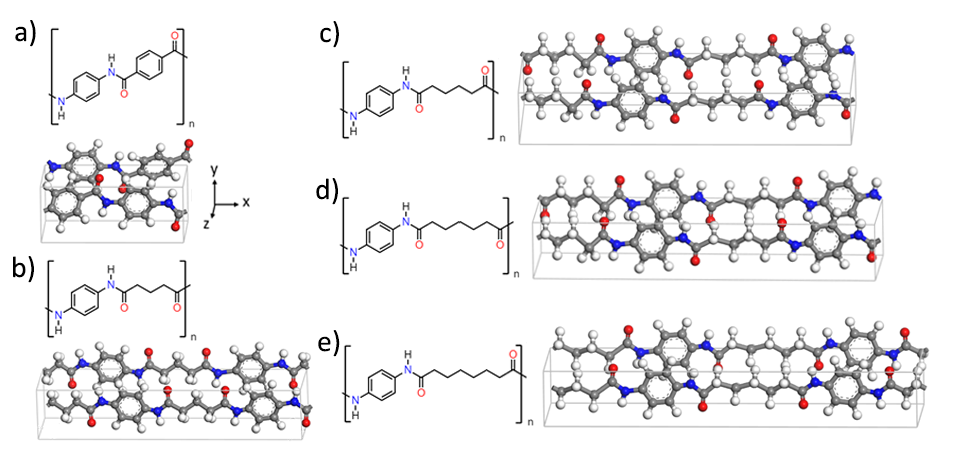
\includegraphics[scale=0.5]{Models.png}
\caption{Unit cells of (a) PPTA, (b) PAP5, (c) PAP6, (d) PAP7, and (e) PAP8. The orthogonal directions (x, y, and z) are defined with respect to the perspective views of the unit cells. Atom colors correspond to: oxygen, red; nitrogen, blue; carbon, gray; and hydrogen, white.}
\label{fig:model}
\end{figure} 

\FloatBarrier
%\subsection{Force Fields}
In our previous study~\cite{yang2021molecular}, two non-reactive force fields (OPLS (Optimized Potentials for Liquid Simulations)~\cite{dodda2017ligpargen} and CVFF (Consistent Valence Force Field)~\cite{Dauber1988Structure}) and seven different ReaxFF parameterizations were tested for PPTA and PAP5.
The results indicated that the ReaxFF force field developed by Liu~\cite{liu2011reaxff} was best for studying structure-property relationships of PPTA and PAP5.
Since the structure of PAP6, PAP7, and PAP8 are similar to PPTA and PAP5, we used the ReaxFF Liu force field for the simulations here. 


%\subsection{Simulation Protocol}
All of the MD simulations were carried out using the open-source MD simulation package LAMMPS (Large-scale Atomic/Molecular Massively Parallel Simulator).~\cite{plimpton1995fast}
Software OVITO (Open Visualization Tool) \cite{stukowski2009visualization} was used for model visualization.
The MD time step was 0.25~fs for all simulations.
Temperature and pressure were controlled using a Nos\'e-Hoover thermostat~\cite{hoover1985canonical} and barostat~\cite{hoover1986constant} with damping parameters of 25~fs and 250~fs, respectively.
Each polymer crystal was equilibrated by running simulations in the NPT (constant number of atoms, pressure and temperature) ensemble for 125~ps (until the lattice parameters reached steady-state) at 300~K and 1~atm.

% Stress-strain Simulations
After equilibration, the system was stretched in the chain direction (x-direction) with a strain rate of 1$\times$10\textsuperscript{9} s\textsuperscript{-1} until the total strain reached 25\%. 
The details of the methods were reported in our previous paper~\cite{yang2021molecular}.
The low-strain elastic modulus was calculated by applying a linear fit to the stress-strain data from 0-2\% strain, and the high-strain modulus was calculated from the last 5\% before failure.
The ultimate stress was the stress at the failure strain.
These simulations were repeated three times independently with different random velocity seeds before NPT simulation.

\FloatBarrier
\section{Results and Discussion}
%\subsection{Elastic Properties}

%\subsubsection{Stress-strain Response and Modulus}
% Describing Observations from the figure
The stress-strain curves for the polyamides are shown in Fig.~\ref{fig:Stress-strain-Curves-and-Modulus}. 
All of the aromatic-aliphatic polyamide crystals exhibit strain hardening, transition from a low-strain linear regime to a high-strain liner regime. 
In Fig.~\ref{fig:Stress-strain-Curves-and-Modulus}b, the low-strain and high-strain moduli are plotted as functions of the number of non-aromatic carbons in the polymers.
We observe that the high-strain modulus is essentially independent of the number of non-aromatic carbon atoms.  This results is supported by the fact that at high strain the modulus is mediated by stretching covalent bonds within the polymer, and the bond stretching and bending stiffnesses are about the same in all five polymers.
\begin{figure}[h!]
\centering
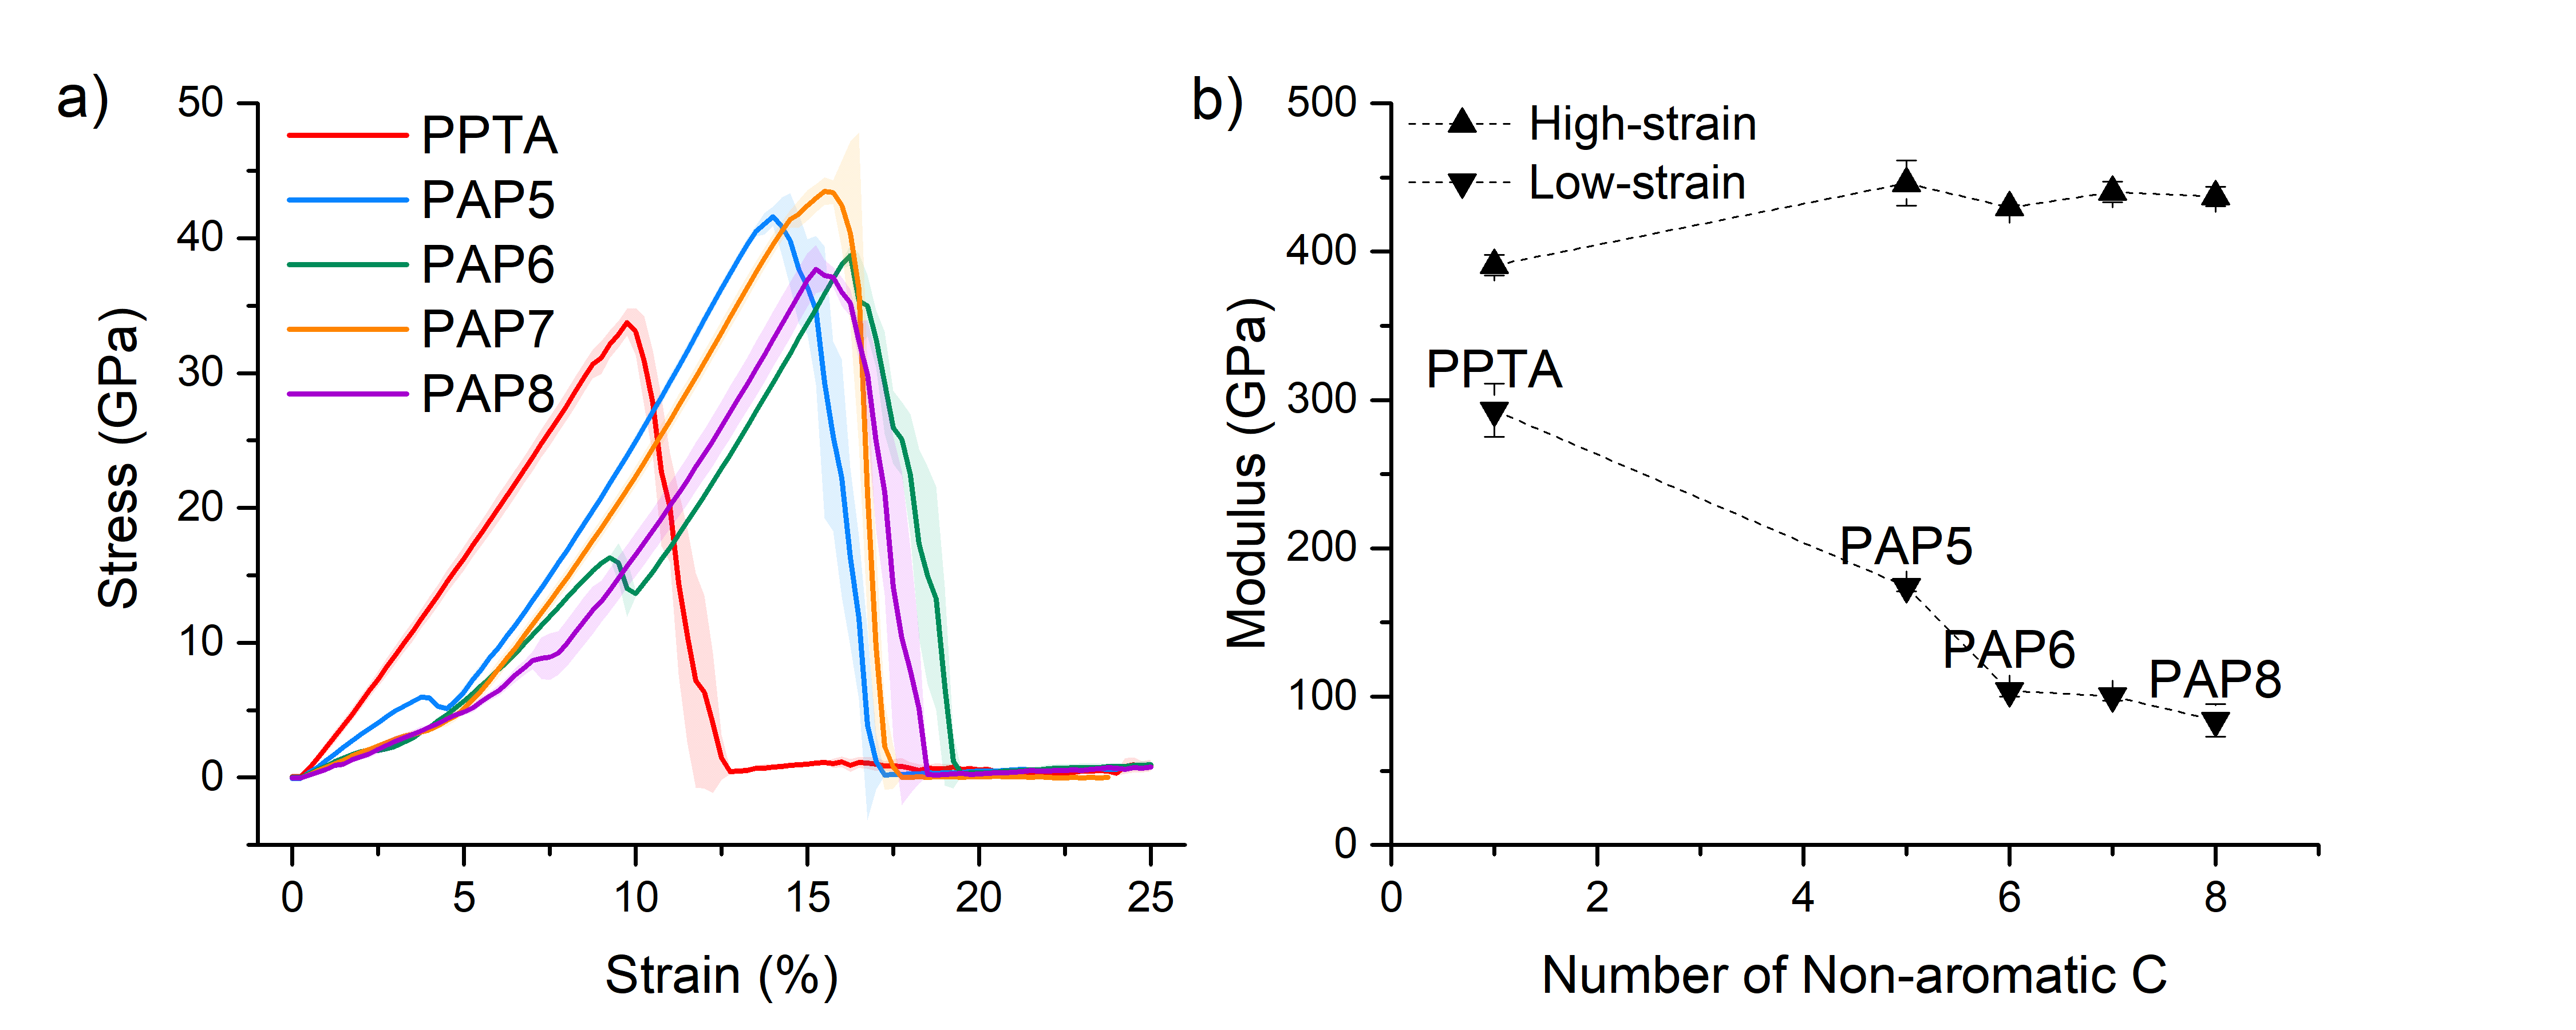
\includegraphics[scale=0.45]{Stress-strain-Curves-and-Modulus.png}
\caption{(a) Stress-strain curves for 4x4x4 polyamide crystals strained from 0 to 25\% strain. The shaded areas reflect standard deviations calculated from three independent simulations. (b) Low-strain and high-strain modulus as functions of the number of non-aromatic carbons in the diacid monomer of each polymer. Low-strain modulus is calculated from the slope of stress-strain curve from 0 to 2\% strain. High-strain modulus is calculated from the last 5\% strain before failure. }
\label{fig:Stress-strain-Curves-and-Modulus}
\end{figure}


% Explanation of the trend of low-strain modulus by waviness
In contrast, the low-strain modulus decreases with increasing number of non-aromatic carbon atoms (Fig.~\ref{fig:Stress-strain-Curves-and-Modulus}b).
In our previous study of PPTA and PAP5,~\cite{yang2021molecular} we found that low strain behavior could be correlated to chain waviness because wavy chains can accommodate strain without stretching covalent bonds.
Waviness can be quantified from the distribution of the atoms in the polymer in the plane transverse to the chain direction, i.e., the y-z plane.
Fig.~\ref{fig:SideView-Waviness-and-Low-strain-Modulus}a is a representative plot of the positions of the non-aromatic backbone atoms in PAP7 with respect to the centroid of each chain, from zero strain to failure.
At low strain (darker blue), the atoms are far from the centroid, indicating a wavy structure.
Then, as strain increases (lighter blue), the chain is extended, and the atoms are found closer to the centroid.


Waviness was then calculated as the radius R of a circle that encompasses 90\% of the atomic coordinates closest to the center of the chain such that a larger radius corresponds to atoms further from the centroid and wavier chain.
% The waviness of all polymer crystals at zero strain was quantified as the radius of the circle fit to the outline of the most-close-to-centroid non-aromatic carbons and nitrogen atoms.
The results for all polymers are shown in Fig.~\ref{fig:SideView-Waviness-and-Low-strain-Modulus}b, where waviness increases with number of non-aromatic carbons.
The increasing trend of waviness is due to the methylene groups acting as spacers between the hydrogen-bonded amide groups, which increases the conformational freedom of the polymer chains.
The low-strain modulus is re-plotted in Fig.~\ref{fig:SideView-Waviness-and-Low-strain-Modulus}b to show that the decrease in modulus corresponds with increasing waviness.

\begin{figure}[h!]
\centering
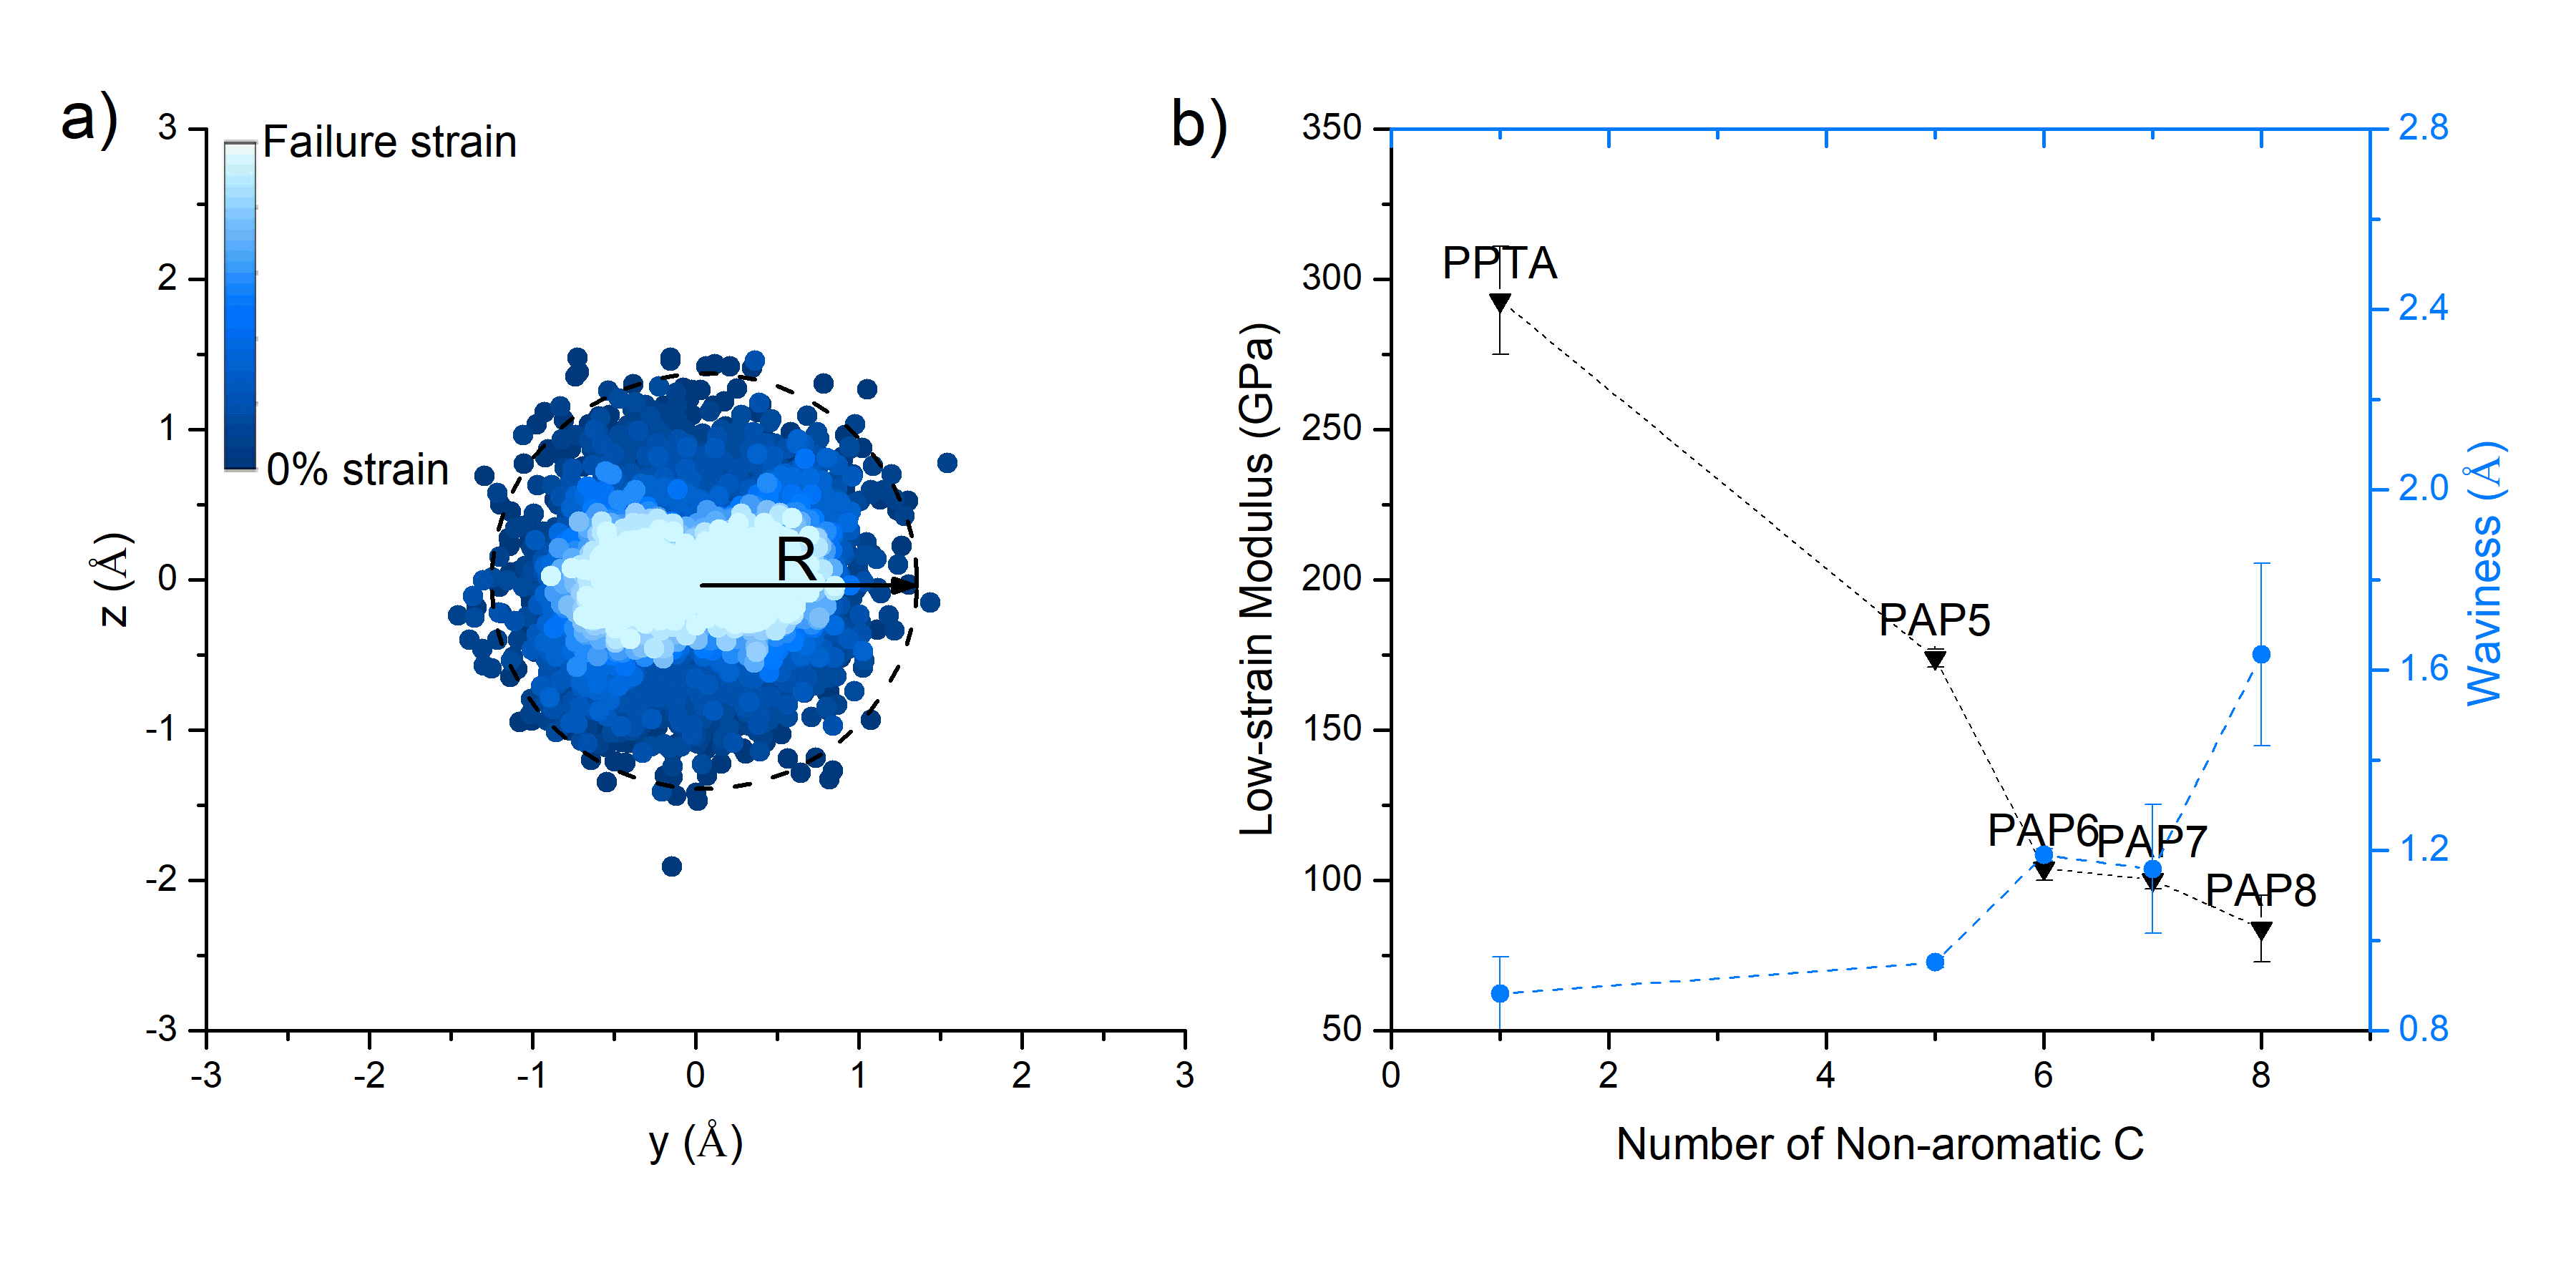
\includegraphics[scale=0.55]{SideView-Waviness-and-Low-strain-Modulus.png}
\caption{(a) Positions of atoms in the chains projected on the yz plane for PAP7 as a function of strain, where the origin corresponds to the centroid of each chain. Similar plots for the other polymers are shown in Fig. S1. The radius R\_0 of a circle encompassing the coordinates of 90\% of the inner-most non-aromatic carbon atoms and nitrogen atoms averaged over three independent simulations is calculated as a measure of waviness. (b) Low-strain modulus and waviness as functions of the number of non-aromatic carbons. The error bars reflect the standard deviations calculated from three independent simulations.}
\label{fig:SideView-Waviness-and-Low-strain-Modulus}
\end{figure}

%\subsubsection{Single Chain and Crystal}
% transition in stress-strain curves
In Fig.~\ref{fig:Stress-strain-Curves-and-Modulus}, except for PPTA, all of the polymers exhibit a transition (inflection) between low and high strain in the stress-strain curve.
Also, for some polymers, there is a sharp shoulder in the stress-strain curve.
However, the shapes and sharpness of these transition points are different for the different polymers.
% a have similarities, differences should be noticed as well, e.g., some (PAP5, PAP6, and PAP8) of the stress-strain curves have a sharper transition than the others (PPTA, PAP7).

% Explanation of transition in stress-strain curves by intra- and inter-chain interactions
To explore the origin of this behavior, stress-strain simulations were performed for single chains taken from the end of the NPT simulation of each crystal.
Two representative comparisons between crystals and single chains are shown in Fig.~\ref{fig:Stress-strain-Curve-SingleChain-vs-Crystal}.
Both single chains and crystals exhibit lower stiffness at low strain than high strain and a gradual increase in stiffness around 5\% strain, indicating that this behavior is due to \textit{intra-chain} processes.
For PAP6 (Fig.~\ref{fig:Stress-strain-Curve-SingleChain-vs-Crystal}a) and PAP8 (Fig. S2), the stress response transitions sharply from low to high strain behavior around 10\% strain, while the single chain does not. 
This indicates that the sharp transition or shoulder in the stress-strain response of some polymers is due to \textit{inter-chain} effects.
 

\begin{figure}[h!]
\centering
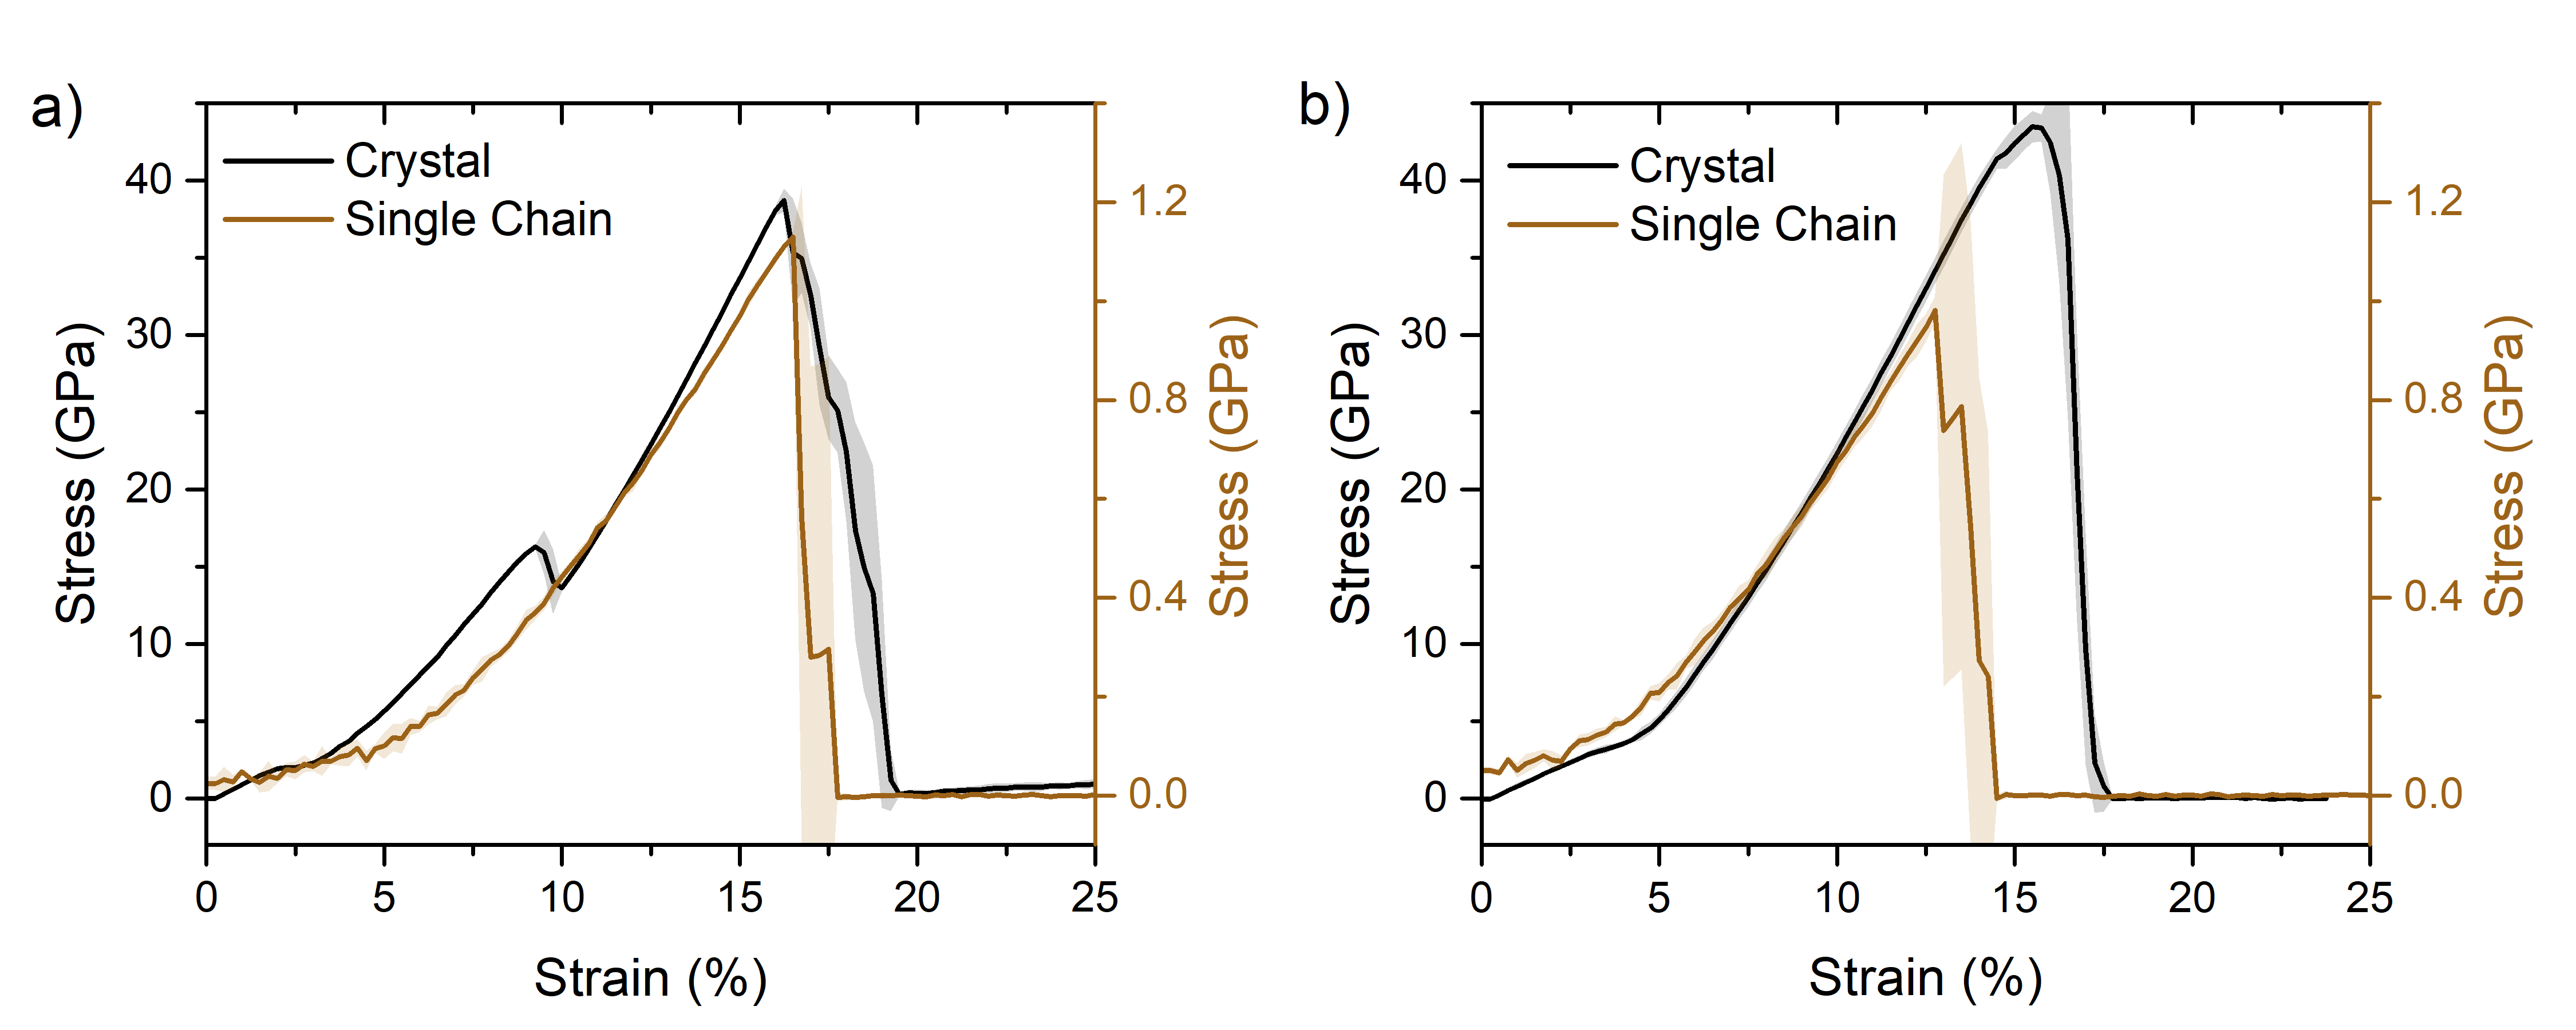
\includegraphics[scale=0.45]{Stress-strain-Curve-SingleChain-vs-Crystal.png}
\caption{Stress-strain response of single chain and crystal forms of (a) PAP6 and (b) PAP7. The single chain is taken from the end of the NPT simulation of each crystal. Similar trends for PAP5 and PAP8 are shown in Fig. S2.}
\label{fig:Stress-strain-Curve-SingleChain-vs-Crystal}
\end{figure}


\FloatBarrier
%\subsubsection{Two Effects in Strain Accommodation}
% introduction to slip and dihedral rotation
To understand how inter- and intra-chain interactions affect the stress-strain response of the crystals, the movement of the atoms and aromatic rings was characterized in terms of inter-chain slip and rotation of dihedral angles.
Inter-chain slip was quantified by the change of average distance in the strain (x) direction between the centers of mass of each pair of adjacent aromatic rings stacked in the z-direction.
Intra-chain dihedral rotation was quantified through three different dihedral angles (HNCO, NCCC, and OCCC) in the backbones.
The results are plotted vs. strain in Fig.~\ref{fig:Slip-and-Rotation-vs-Strain}.
 
% intra-chain interactions
The motions are quantified by the change of dihedral angles during stretching relative to the equilibrated state at zero strain.
For PAP5-PAP8, the NCCC dihedral angle increases and the OCCC angle decreases gradually in the low-strain regime as the energy barriers for bond rotations are overcome.~\cite{tonelli2020poly} 
The gradual increase in stiffness in the low-strain regime exhibited by all polymers, except PPTA, correlates well with changes in the dihedral angles (i.e., decreasing OCCC angle and increasing NCCC angle), indicating the low strain is accommodated by straightening wavy chains.
Then, when the chain is fully extended, the angles increase/decrease abruptly and remain at a constant value until failure.  
The strain at which these rotational modes are exhausted corresponds closely with the transition out of the low-strain regime for all four aromatic-aliphatic polyamides.

% inter-chain interactions
The predominant inter-chain mechanism observed in the simulations is slip between chains.
At zero strain, the rings of all five polymers are in nearly perfect registry along the x-coordinate, i.e., "slip" is near zero.
For PPTA, PAP5, and PAP7, the slip remains at zero until failure.
However, for PAP6 and PAP8 (animations in Movie S1), the chains undergo a discrete slipping event (the magnitude of which is only ~0.5 A) at the transition between low and high-strain behavior, i.e., the transition between the wavy and extended conformation.
After this slip event, the relative position of the crystal stems remains stable until failure.
This slip mechanism is accessible to PAP6 and PAP8 because they have an even number of carbon atoms, which corresponds to a parallelogram structure that is less stable than the trapezoid structure of polymers with an odd number of carbon atoms ~\cite{thalladi2000melting,white2008room,bond2004crystal}(see Fig. S3 for representative snapshots of these structures).
This so-called odd-even effect~\cite{baeyer1877ueber,thalladi2000melting} has been observed in the elastic properties of polymers including $\alpha$,$\omega$-alkanedicarboxylic acids~\cite{mishra2013odd} and polyesters~\cite{shen2017facile}.
\begin{figure}[h!]
\centering
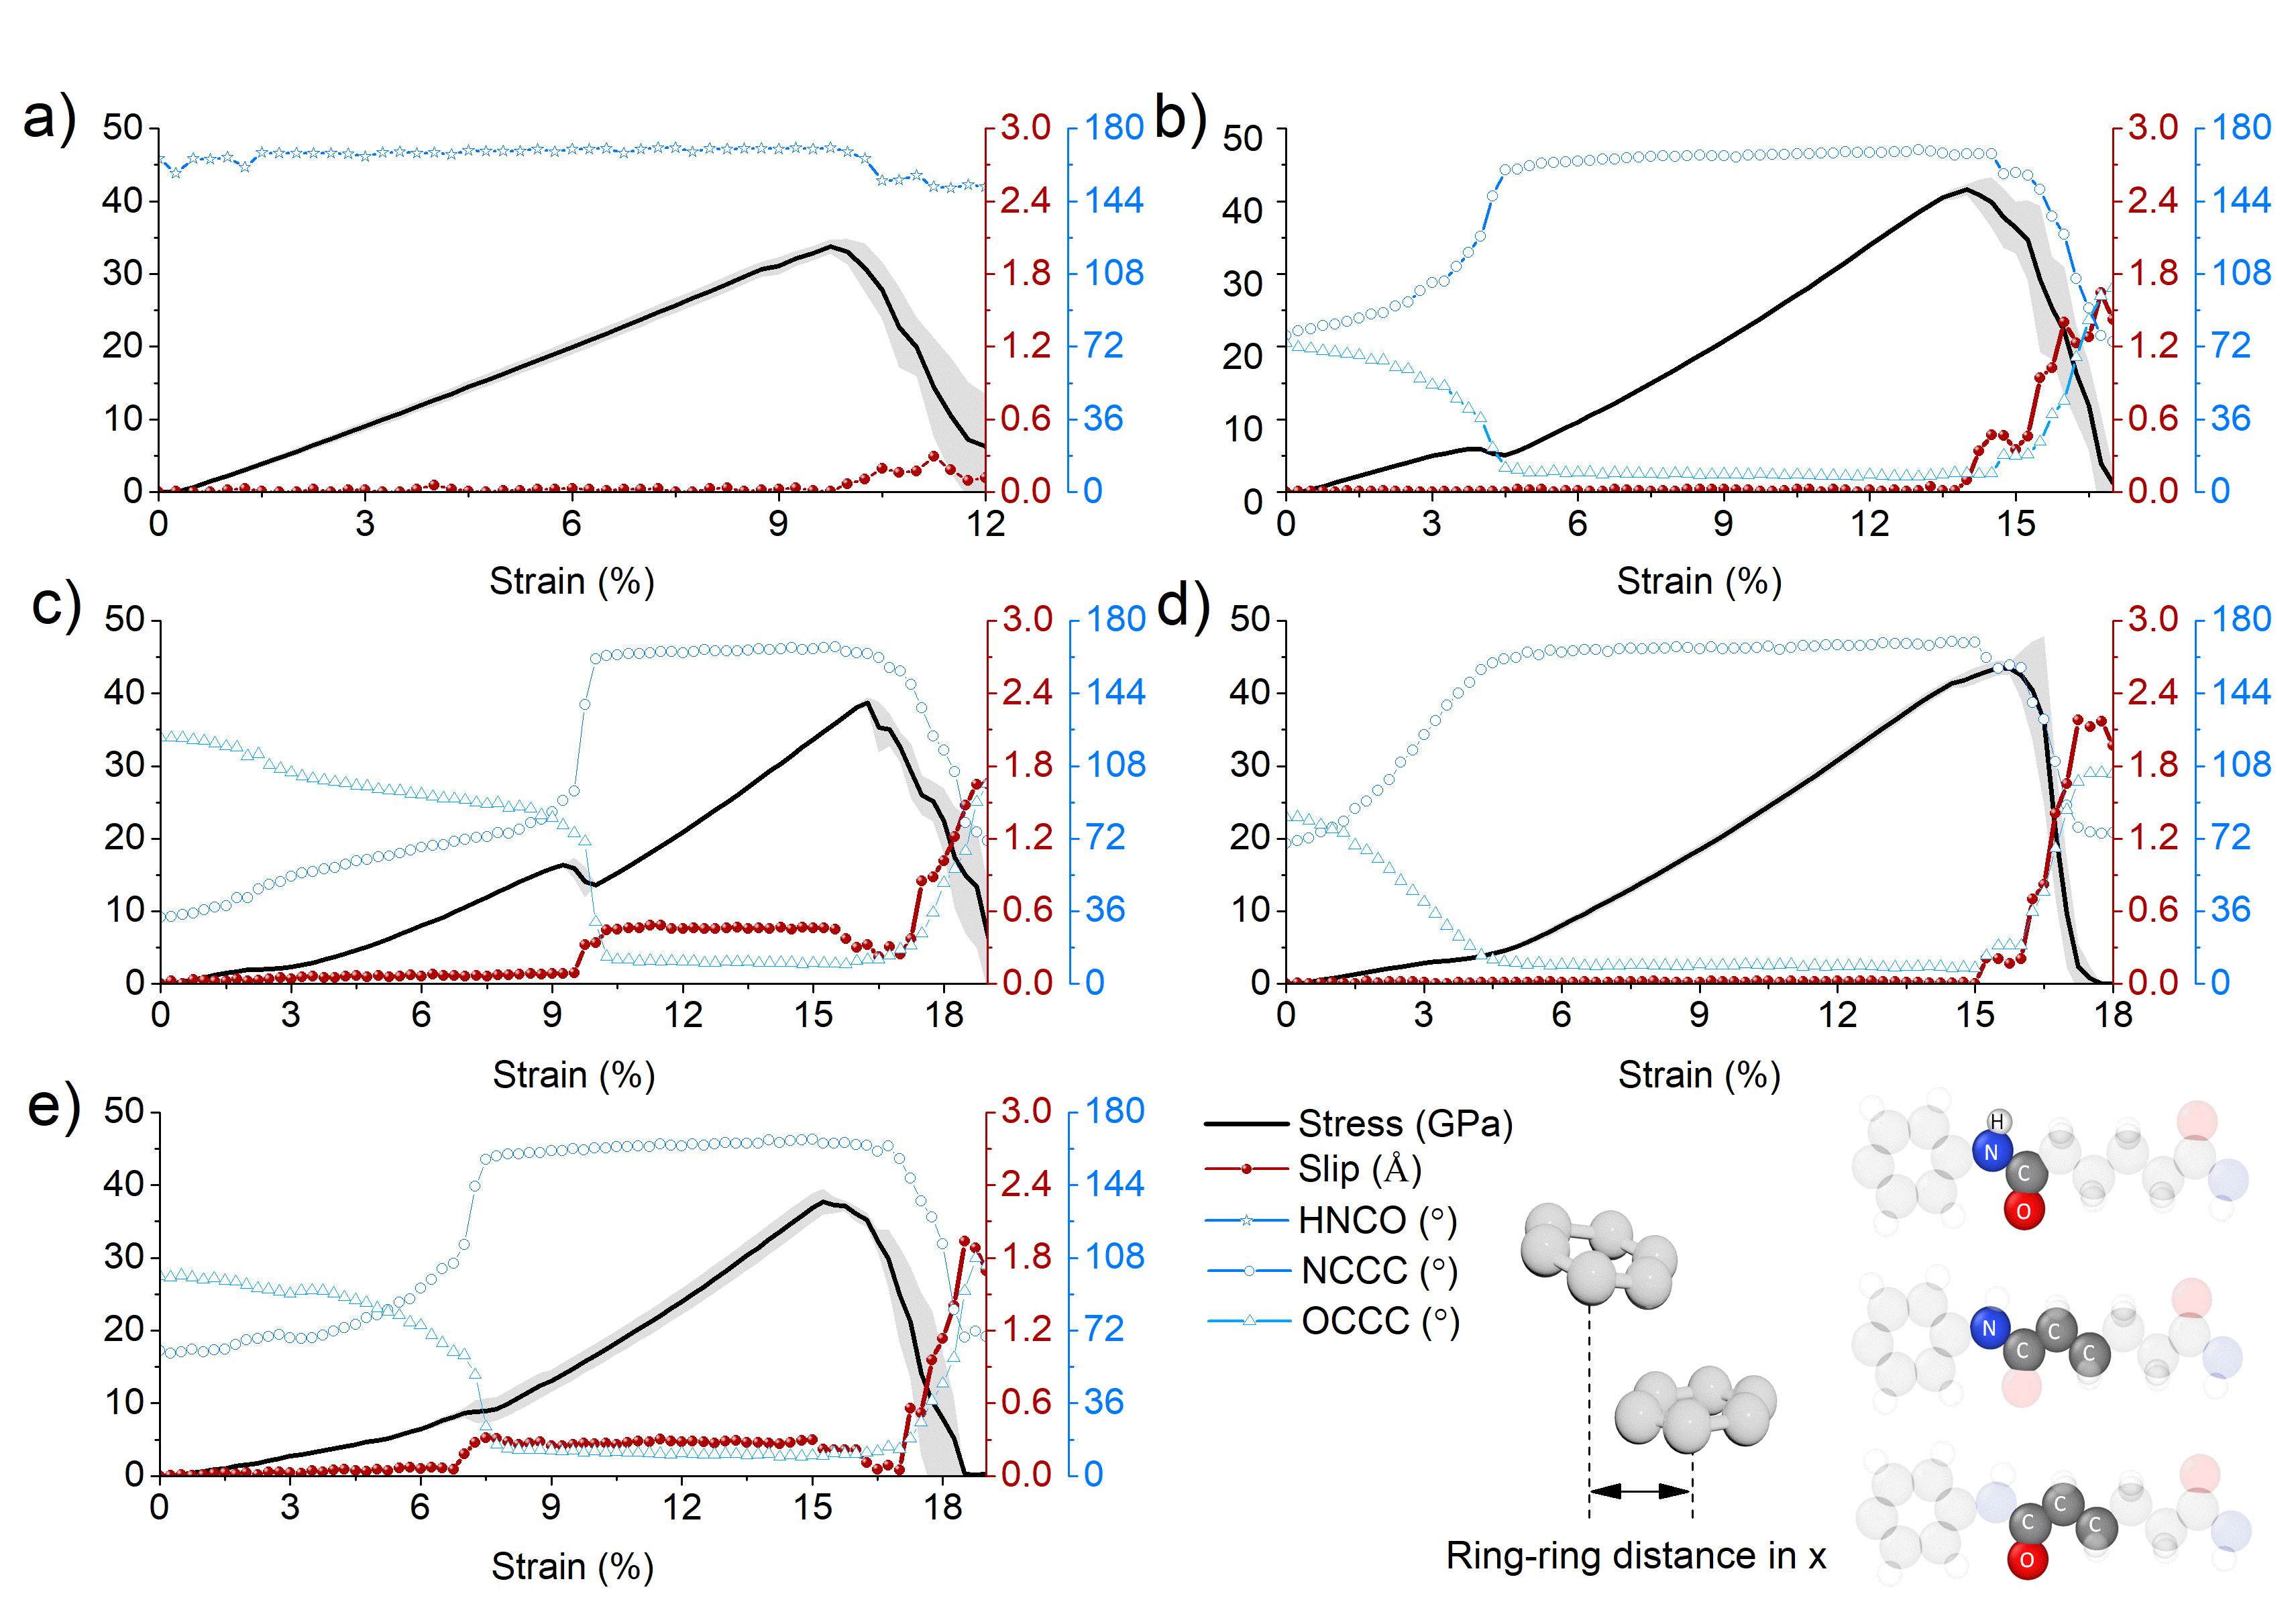
\includegraphics[scale=0.55]{Slip-and-Rotation-vs-Strain.png}
\caption{Stress, inter-chain slip, and dihedral angles as functions of strain of (a) PPTA, (b) PAP5, (c) PAP6, (d) PAP7, and (e) PAP8.}
\label{fig:Slip-and-Rotation-vs-Strain}
\end{figure}



\FloatBarrier
%\subsection{Ultimate Properties}
%\subsubsection{Ultimate Stress and Coplanarity of Aromatic Rings}
% description of trends of ultimate stress in Figure 6

Odd-even effects have also been observed in the ultimate properties of polyurethane
elastomers~\cite{prisacariu2011influence} and polyesters~\cite{shen2017facile}.
%The analysis so far has focused on the elastic response of the polymer crystals.
As shown in Fig.~\ref{fig:Coplanarity}, aromatic-aliphatic polyamides with an even number of carbon atoms have lower ultimate stress.
In all cases the reactive simulations predict that failure occurs by breaking the N-C(O) bond in the amide.
Density functional theory (DFT) calculations were used to probe the bond dissociation energies (BDEs) of the N-C(O) in single repeat units of PPTA and a representative fragment of an aromatic-aliphatic polyamide (Fig. S4).  
The DFT results showed that the aliphatic segment does not affect bond strength, suggesting the observed odd-even trend in ultimate stress is an inter-chain effect.
%The ultimate stress, reported in Fig.~\ref{fig:Coplanarity}, is lower for PPTA than the other polymers, indicating an improvement of tensile strength due to the introduction of methylene units.
%In addition, among the four methylene-containing polymers, there is odd-even behavior, where polymers with an even number of carbon atoms have lower ultimate stress.
% First, the slip exhibited by PAP6 and PAP8 (Fig.~\ref{fig:Slip-and-Rotation-vs-Strain}) likely contributes to their lower ultimate strength.


% Analysis of coplanarity; explain odd-even effect by coplanarity of rings
It has been shown that ring-ring interactions ($\pi$-stacking) affect the ultimate properties of polyamides, and the strength of these interactions is related to the coplanarity of the rings.~\cite{yang2021molecular,burattini2011supramolecular}
The coplanarity of the rings is quantified here by the angle between each pair of aromatic rings in adjacent chains (see inset to Fig.~\ref{fig:Coplanarity}) averaged over the last 2\% strain before failure. 
Coplanarity is plotted as a function of the number of non-aromatic carbons in Fig.~\ref{fig:Coplanarity}, where small ring-ring angle corresponds to better registry between the aromatic rings (high coplanarity).
The ultimate stress and coplanarity of the polymers exhibit consistent trends where polymers with poorer registry (weaker $\pi$-$\pi$ interactions) and lower strength.
%This correlation between coplanarity and ultimate stress is consistent with our previous study on PPTA and PAP5 that reported better coplanarity indicates stronger ring-ring interaction therefore higher ultimate stress.~\cite{yang2021molecular} 

% Inter-chain Slip
%In addition to coplanarity of aromatic rings, the inter-chain slip observed for the even polymers is also a reason for the smaller ultimate stress of the even polymers.
%The slip lower the alignment of the aromatic rings in the y-direction (Movies S1) further which further decrease the inter-chain interactions and chain regularity of even polymers. 


\begin{figure}[h!]
\centering
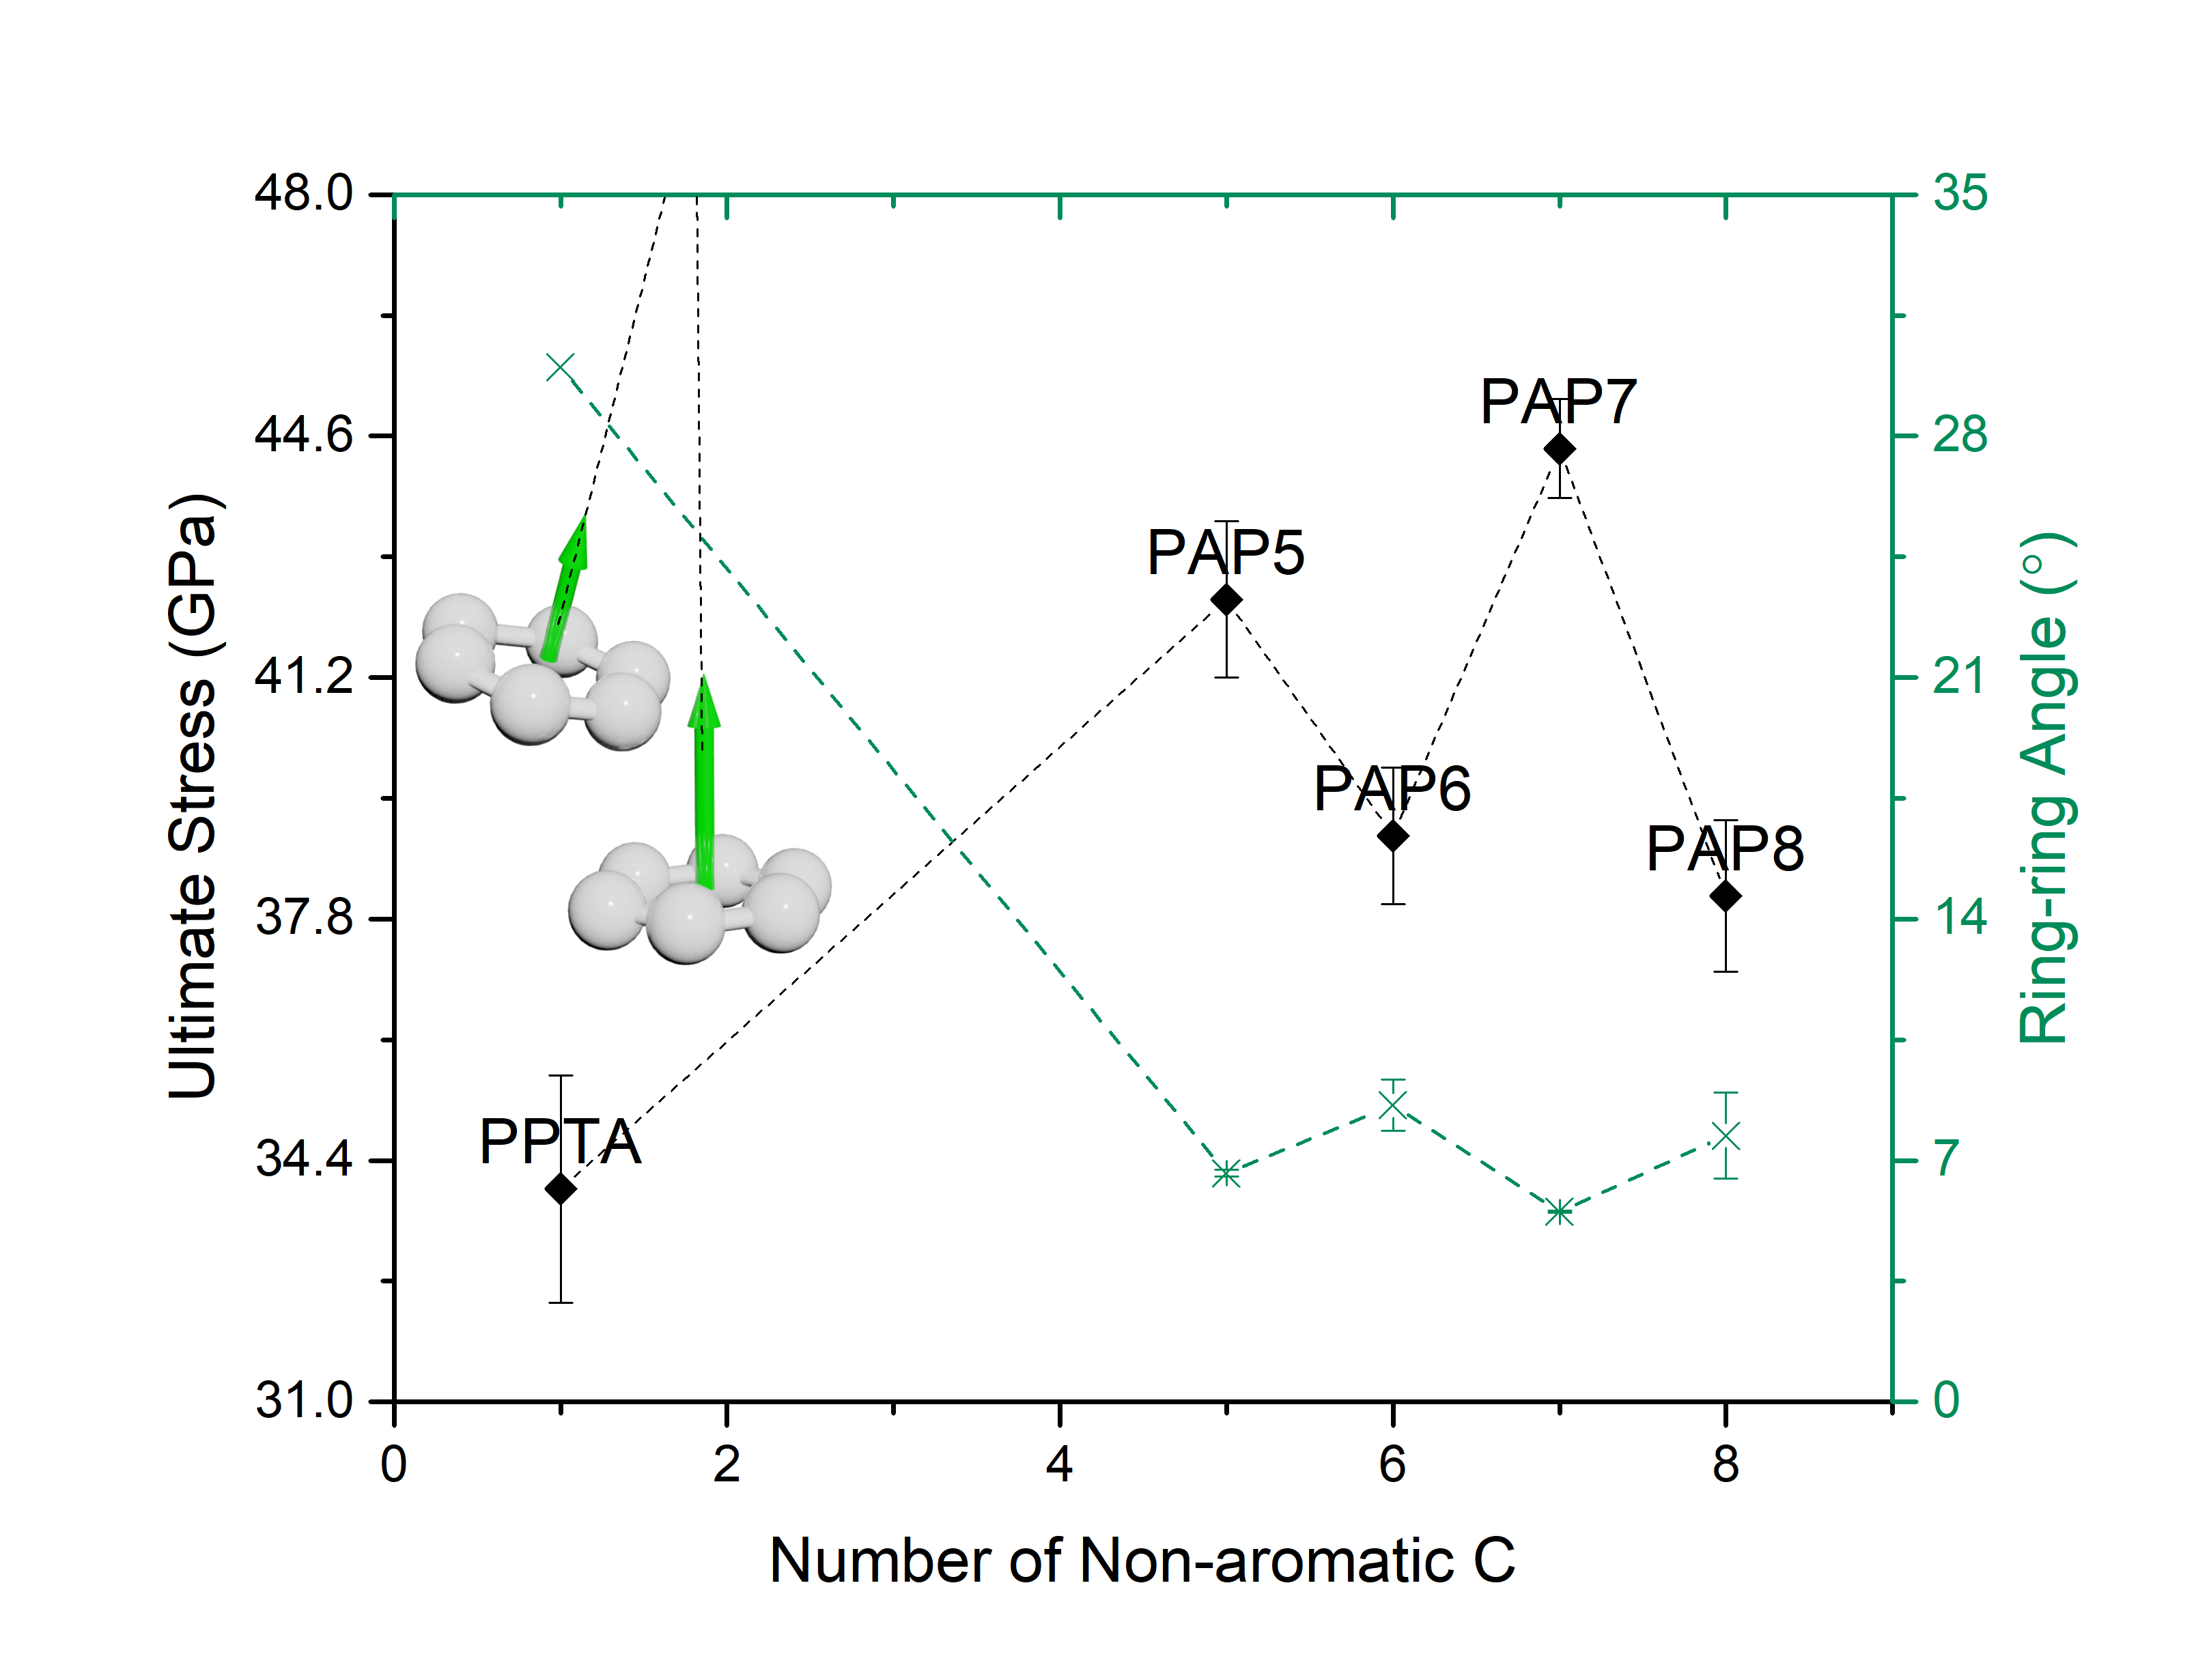
\includegraphics[scale=0.60]{Coplanarity.png}
\caption{Ultimate stress and coplanarity, quantified by the ring-ring angle, as functions of the number of non-aromatic carbons. The errors bars reflect the standard deviation from three independent simulations.}
\label{fig:Coplanarity} 
\end{figure}



\FloatBarrier
\section{Conclusions}
% General description of what were done
Molecular dynamics simulations were performed to study the stress-strain response of PPTA and four related aromatic-aliphatic polyamides with different numbers of non-aromatic carbons in the aliphatic chain. 
Two distinct linear stress-strain regimes were observed.
% General description of the results
It was found that the subtle structural differences between these polymers lead to distinct elastic and ultimate properties.
% Results of elastic properties
The low-strain modulus (calculated from 0-2\% strain) decreased with increasing aliphatic chain length while the high-strain modulus (calculated from the last 5\% strain before failure) was independent of the aliphatic chain length.
% Explanation of the elastic properties
The trend of low-strain modulus was explained in terms of departure from the extended chain conformations--waviness-- of the polymers at zero strain.
Longer aliphatic chain length increased the conformational freedom of the chains and therefore increased the waviness of the polymers, which finally decreased the low-strain modulus.
% Results of transition between low- and high-strain
The transition from low to high strain behavior was correlated to rotation of dihedral angles as the chains were extended, so this behavior was due to intra-chain effects.
It was also observed that polymers with an even number of carbon atoms
%in the alphatic chain exhibited a sharp transition between low-strain and high-strain, while the others had a smoother transition.
% Explanation of transition
exhibited a discrete inter-chain slip mechanism at the transition between the wavy and extended conformation, which was explained by the instability of the trapezoidal structure of these polymers.
%The intra-chain interactions that accommodated strain slowly included elongation of the chain and rotation of dihedrals, which were found for all polymers. 
%In addition, inter-chain slip, which was only found for even polymers, enhanced the sharpness of the transition which explains the larger sharpness of even polymers than the odd counterparts. 
% Results of ultimate property
A similar odd-even effect was observed at failure, where even polymers had lower ultimate stress.
% Explanation of ultimate property 
Coplanarity of the aromatic rings correlated well with the trend of ultimate stress, i.e., less coplanar rings (larger ring-ring angle) corresponded to lower ultimate stress.
%In addition, the inter-chain slip due to the less stable trapezoidal structure of the even polymers was also a main factor for explaining the lower ultimate stress of the even polymers.
% Closure
The results reported here show that aromatic-aliphatic polyamides can be designed with mechanical properties comparable to or better than PPTA yet even subtle differences in chemical composition can affect the mechanical response.
Further, the correlations between structure and mechanical properties identified, as well as the simulation-based approach, may be extended to other similar polymers to enable tuning of mechanical properties through chemical modification.

%
%%%%%%%%%%%%%%%%%%%%%%%%%%%%%%%%%%%%%%%%%%%%%%%%%%%%%%%%%%%%%%%%%%%%%
%% The "Acknowledgement" section can be given in all manuscript
%% classes.  This should be given within the "acknowledgement"
%% environment, which will make the correct section or running title.
%%%%%%%%%%%%%%%%%%%%%%%%%%%%%%%%%%%%%%%%%%%%%%%%%%%%%%%%%%%%%%%%%%%%%
\begin{acknowledgement}
We acknowledge ExxonMobil Research and Engineering Company for financial support of this work. The stimulating discussions with ExxonMobil colleagues (Ozcan Altintas, Arben Jusufi, Aruna Mohan, Agostino Pietrangelo, Thomas Sun, Loan T. Vo, Pamela J Wright) are highly appreciated. The simulations were in part run using the Extreme Science and Engineering Discovery Environment (XSEDE), which is supported by National Science Foundation Grant ACI-1548562.
\end{acknowledgement}

%%%%%%%%%%%%%%%%%%%%%%%%%%%%%%%%%%%%%%%%%%%%%%%%%%%%%%%%%%%%%%%%%%%%%
%% The same is true for Supporting Information, which should use the
%% suppinfo environment.
%%%%%%%%%%%%%%%%%%%%%%%%%%%%%%%%%%%%%%%%%%%%%%%%%%%%%%%%%%%%%%%%%%%%%

\FloatBarrier


\pagebreak

\beginsupplement

\section{Supporting Information}

Movie M1: Animation of strain simulations of all polymers shown from the y-direction (H-bond direction) where all atoms except the aromatic rings are faded to highlight the inter-chain slip.

\noindent Movie M2: Animation of strain simulations of all polymers shown x-direction where all atoms except the aromatic rings are faded to highlight the inter-chain slip.



\begin{figure}[h!]
\centering
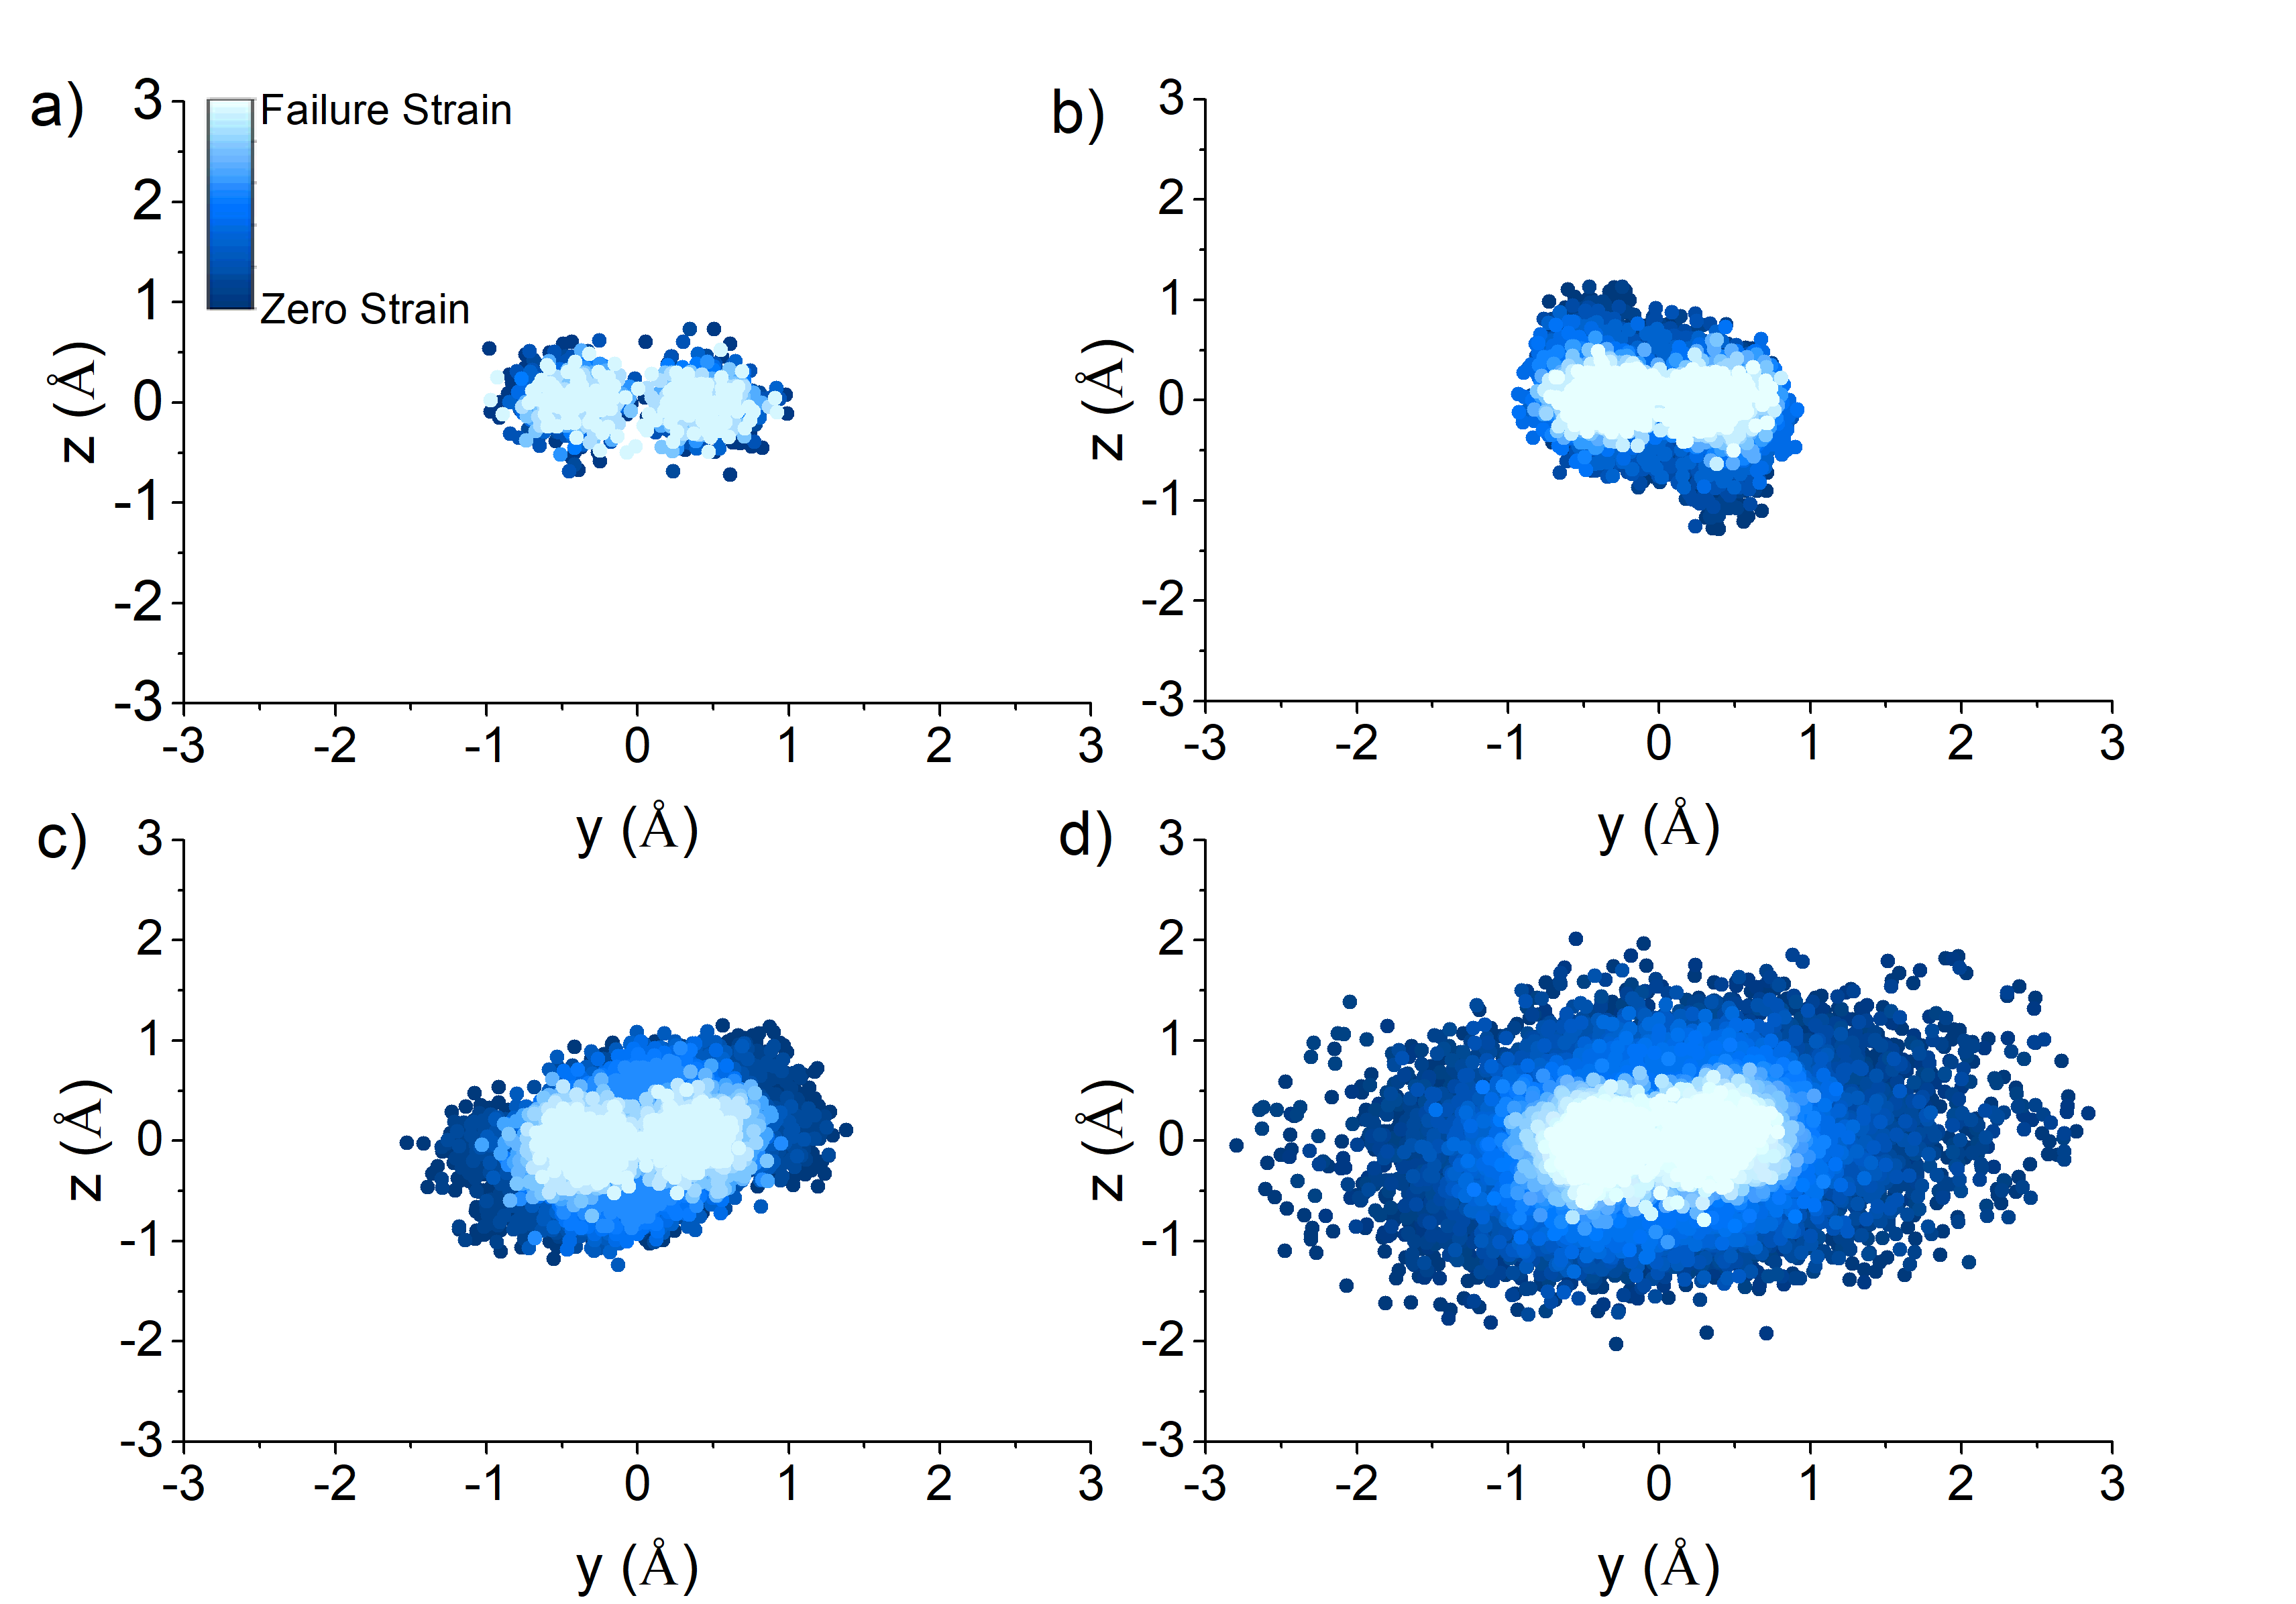
\includegraphics[scale=0.55]{Figure S1 sideviews.png}
\caption{Positions of the non-aromatic, backbone atoms in the chains projected on the yz plane, where the centroid of each chain is the origin of the yz plane, for (a) PPTA, (b) PAP5, (c) PAP6, and (d) PAP8. The radius of a circle fit to the outline of the 90\% innermost non-aromatic carbon atoms is averaged over three independent simulations to quantify waviness. 
}
\label{fig:sideviews}
\end{figure}

\begin{figure}[h!]
\centering
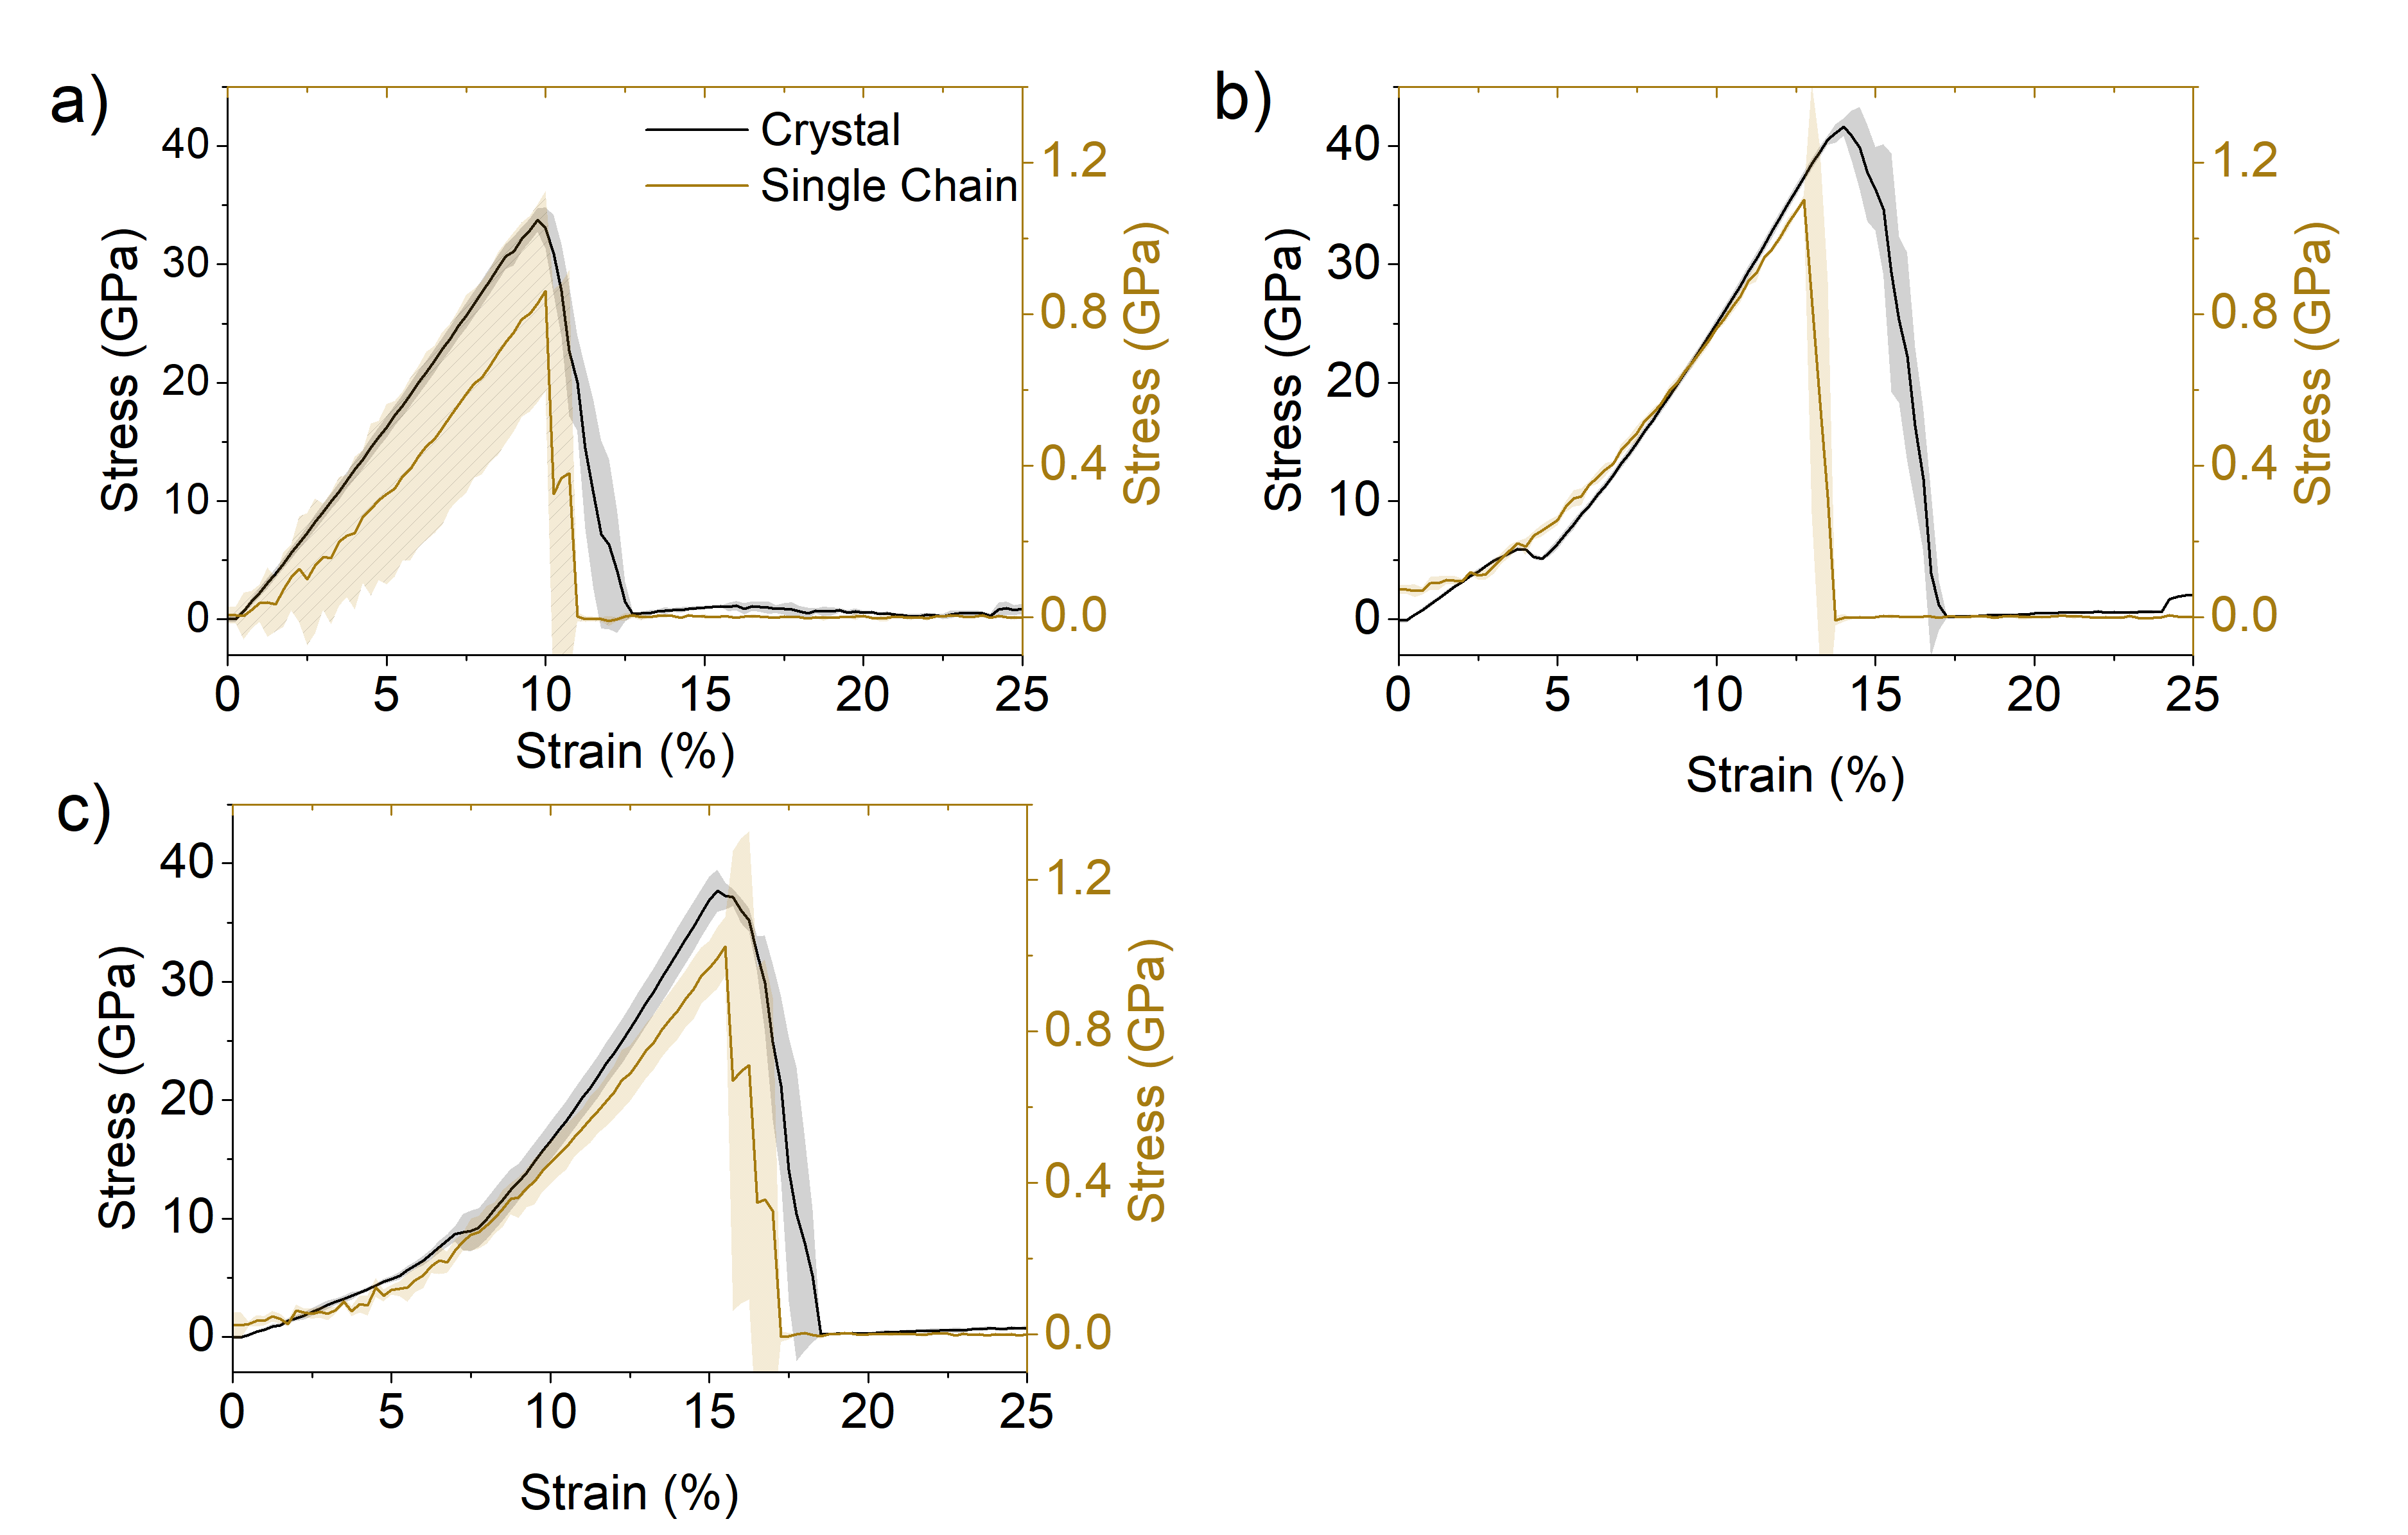
\includegraphics[scale=0.55]{Figure S2 SingleAndCrystal-PPTA-PAP5-PAP8.png}
\caption{Stress-strain response of single chains and crystal forms of (a) PPTA, (b) PAP5, and (c) PAP8. The single chain is taken from the end of the NPT simulation for each crystal.
}
\label{fig:SingleAndCrystal-PPTA-PAP5-PAP8}
\end{figure}


\begin{figure}[h!]
\centering
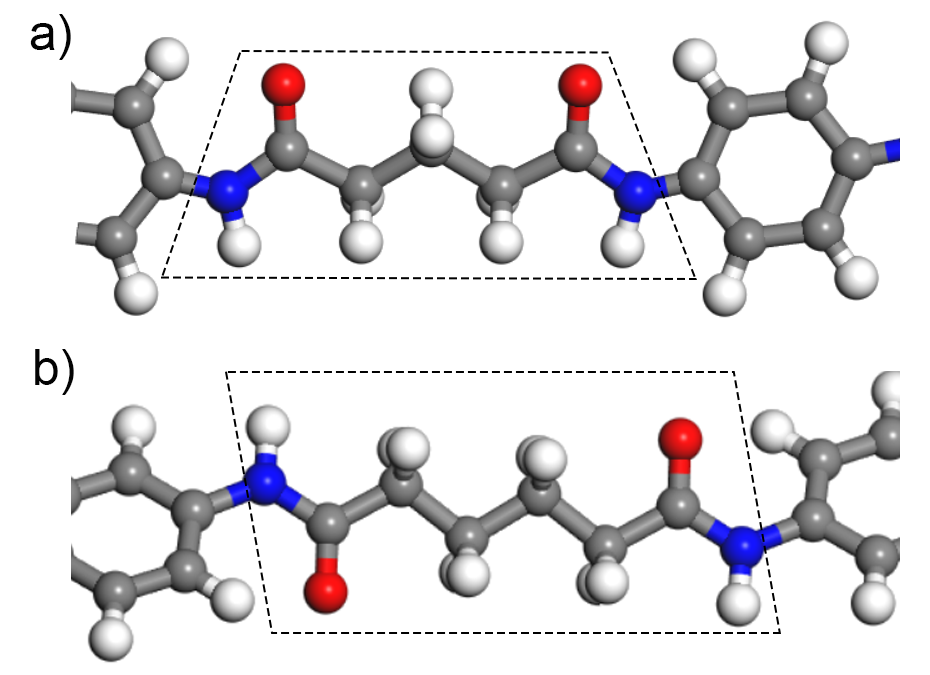
\includegraphics[scale=0.35]{Figure S3 Parallelogram and Trapezoid.png}
\caption{Representative snapshots of trapezoid and parallelogram structures in the backbones of (a) odd (PAP5) and (b) even (PAP6) polymers. 
}
\label{fig:ParallelogramANDTrapezoid}
\end{figure}

\FloatBarrier
\subsection{DFT-computed bond dissociation energy for PPTA and PAP5}

\begin{figure}[h!]
\centering
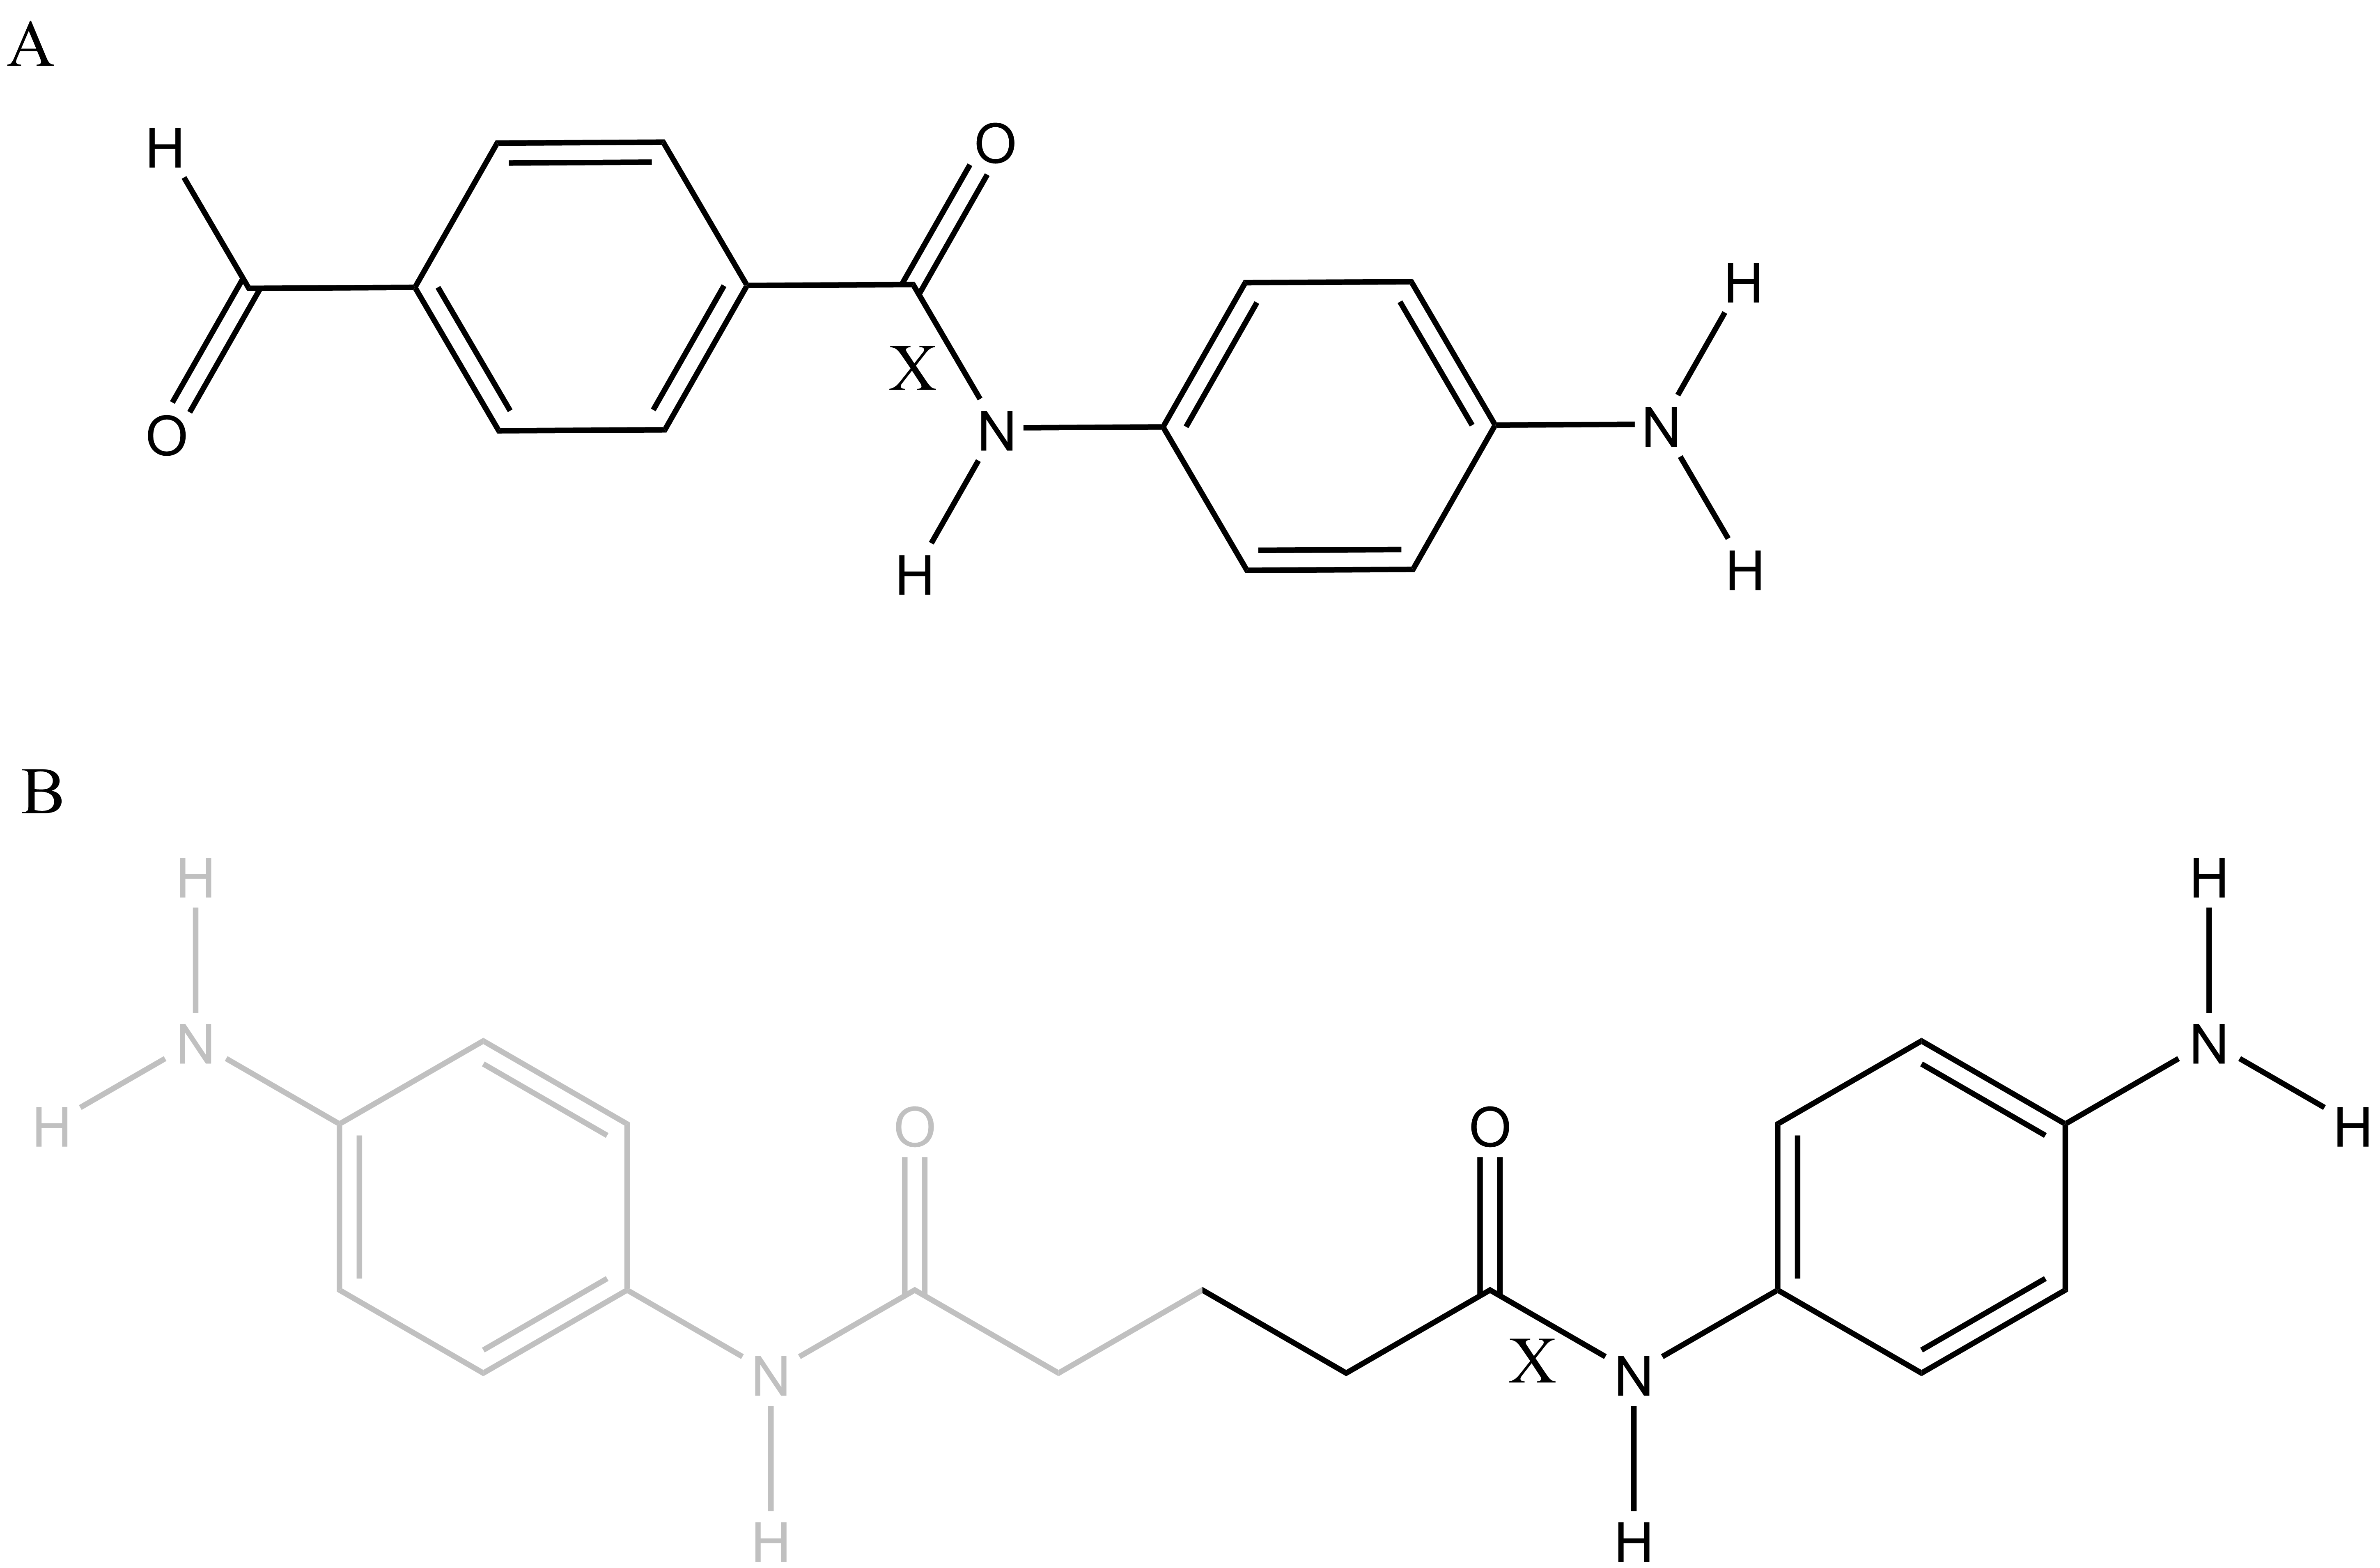
\includegraphics[width=0.8\textwidth]{DFT_figure_chemdraw.png}
\caption{Truncated polymer models used to compute the bond dissociation
energy (BDE) for (a) PPTA and (b) representative aromatic-aliphatic polyamide fragment.
X denotes the bond for which the BDE was computed.
For PAP5, the gray part of the repeat unit was omitted from the DFT calculations
because the cleaved bond is not likely to be affected by more distant
moieties.
}
\label{fig:DFT}
\end{figure}

Fig.~\ref{fig:DFT} shows the model systems used to compute the 
lowest BDE of the polymer chains for PPTA and PAP5.
The bond denoted X was selected based on previous work 
that showed this bond was the weakest in the PPTA system \cite{mercer2017molecular}.
To determine the BDE, the bond X was homolytically cleaved leaving
two fragments each containing an unpaired electron (doublets).
The BDE is then computed from the
difference in Gibbs Free Energy between the whole
molecule and the sum of the fragments.
These calculations were performed in Gaussian 09 \cite{g09}
at the M062X/6-311+G(2d,p) level of theory \cite{zhao_2008,mclean_1980}.

The computed BDE of bond X was 55.7 kcal/mol for PPTA and
56.3 kcal/mol for PAP5.
The 0.6 kcal/mol difference between these two results is
within the expected error of this method, which indicates
their BDE is nearly equivalent.
This calculation was not repeated for PAP6, PAP7, and PAP8 because
the longer aliphatic linker in these polymers is not likely to affect the BDE of bond X.

%%%%%%%%%%%%%%%%%%%%%%%%%%%%%%%%%%%%%%%%%%%%%%%%%%%%%%%%%%%%%%%%%%%%%
%% The appropriate \bibliography command should be placed here.
%% Notice that the class file automatically sets \bibliographystyle
%% and also names the section correctly.
%%%%%%%%%%%%%%%%%%%%%%%%%%%%%%%%%%%%%%%%%%%%%%%%%%%%%%%%%%%%%%%%%%%%%
Test
Test Overleaf Again
\FloatBarrier
\bibliography{ref}





\end{document}


